This chapter presents the results achieved by the chosen methods introduced in Chapter \ref{section::methodology}. The results achieved by each method are collected under the following subchapters respectively. This chapter provides answers to RQ2 and RQ3 (Chapter \ref{section::introduction}).

\subsection{Exploratory Data Analysis}
\label{section::exploratory-data-analysis}
    % unique voters
    By the end of 2017, there is a total number of 573 contests in the platform. To identify what kind of content that is more engaging (RQ2), first let us look at the amount of unique voters over the number of contests. Figure \ref{user_engagement_in_contests} displays a histogram and a boxplot of the number of contests and the number of unique voters that they have engaged. 
    
    \begin{figure}[h] 
        \begin{center}
            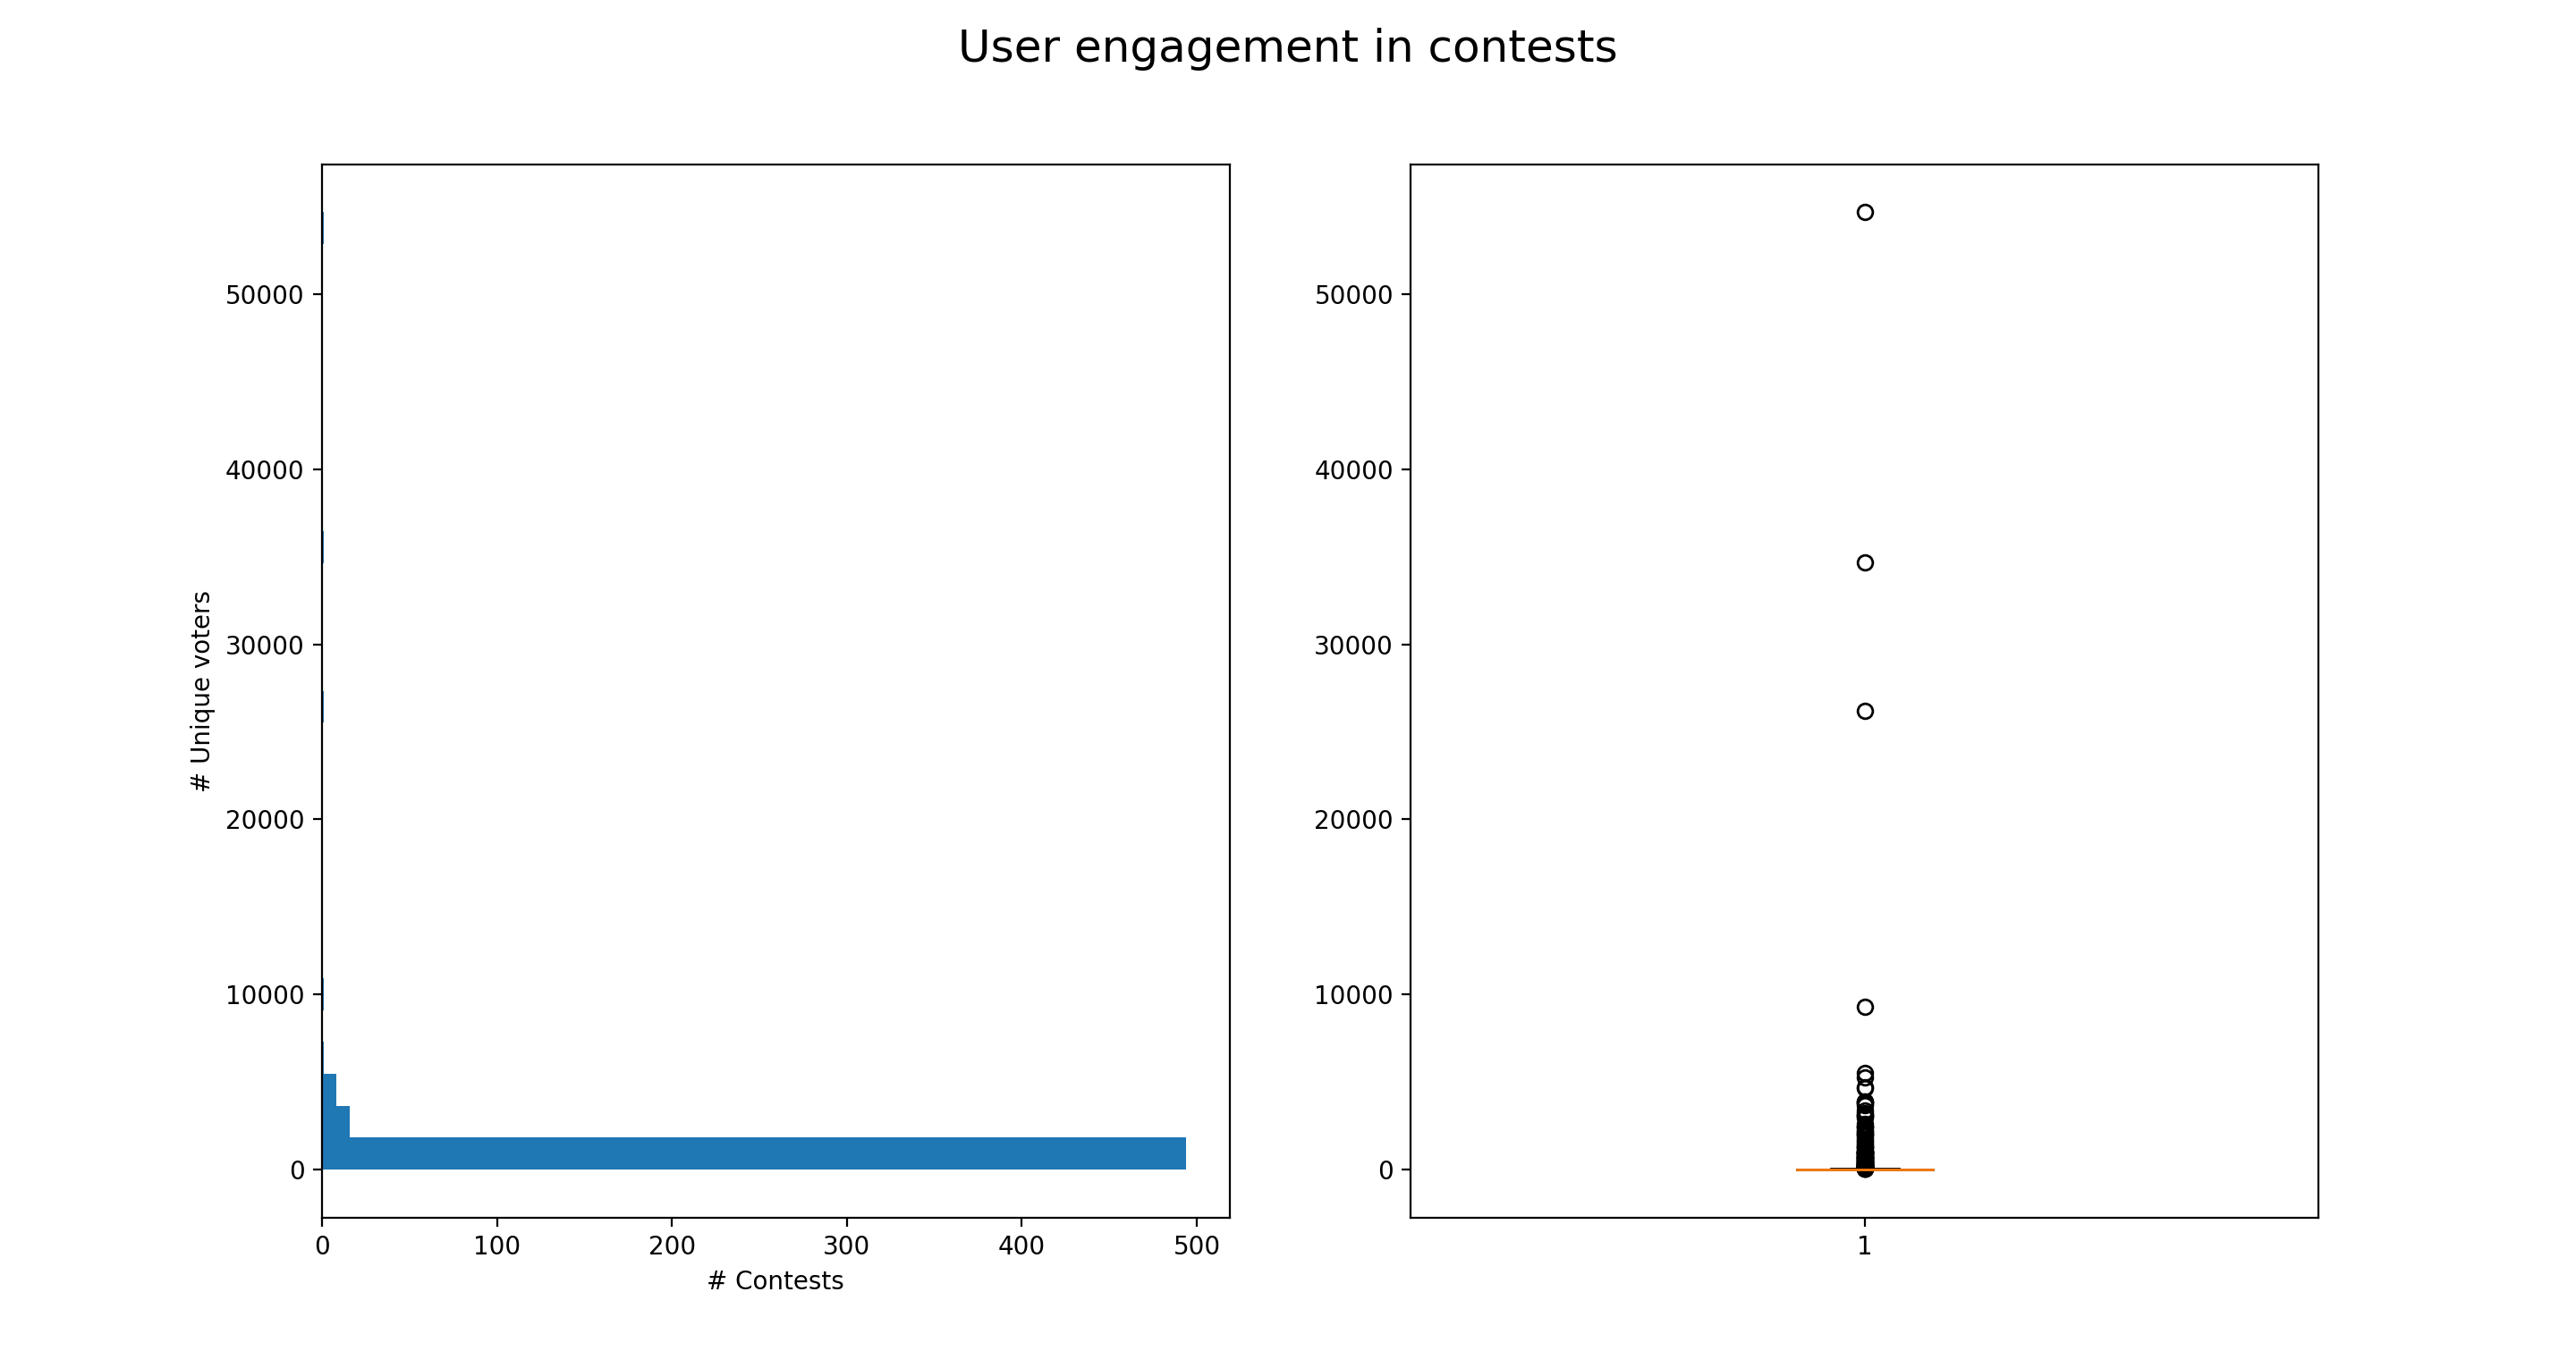
\includegraphics[width=0.8\textwidth]{Images/user_engagement_in_contests.png}
            \caption{The number of unique voters over contests.}
            \label{user_engagement_in_contests}
        \end{center}
    \end{figure}

    It can be easily seen that most of the contests engage very small amount of users, as the median of the unique voter count for all contests is 3. One of the reasons behind this is that the company did not establish a large user base yet. Therefore there are many users who created only one contest but never used the platform on the long run. Many of the contests serve only testing purposes, hence engage only a few users. Such records can create bias in the upcoming analyses, because their data does not represent realistic scenarios. For this reason, contests with less than $100$ unique voters are excluded in the remainder of the analysis, because such observations are not representative. This dataset contains $166 808$ vote transactions by $145 000$ users over $81$ contests, $1 113$ contest participants and $432$ labels on the images recognized by Google Vision. For the remainder of the EDA, this filtered dataset is used.

    Figure \ref{user_engagement_in_contests-pruned} displays the same distribution for the filtered set of contests. In this figure contests with more voters are more apparent. The highest number of unique voters is close to $55 000$ in one of the contests, the mean value ($\mu = 455.43$) and the standard deviation ($\sigma = 3 017.51$). These numbers mean that there is a large variance in the amount of engaged users in contests. It cannot be clearly said which traits make a contest more attractive to users.
    
    The boxplot on the right side of the figure uses the $95$ percentile (around $5 200$ unique voters), above which the outliers can be seen. It can be also seen that the most of the contests engage $260-2 600$ unique voters (as described by the first and the third quartiles). There are $6$ large contests, from which the biggest have engaged $54 684$ voters. 

    \begin{figure}[h] 
        \begin{center}
            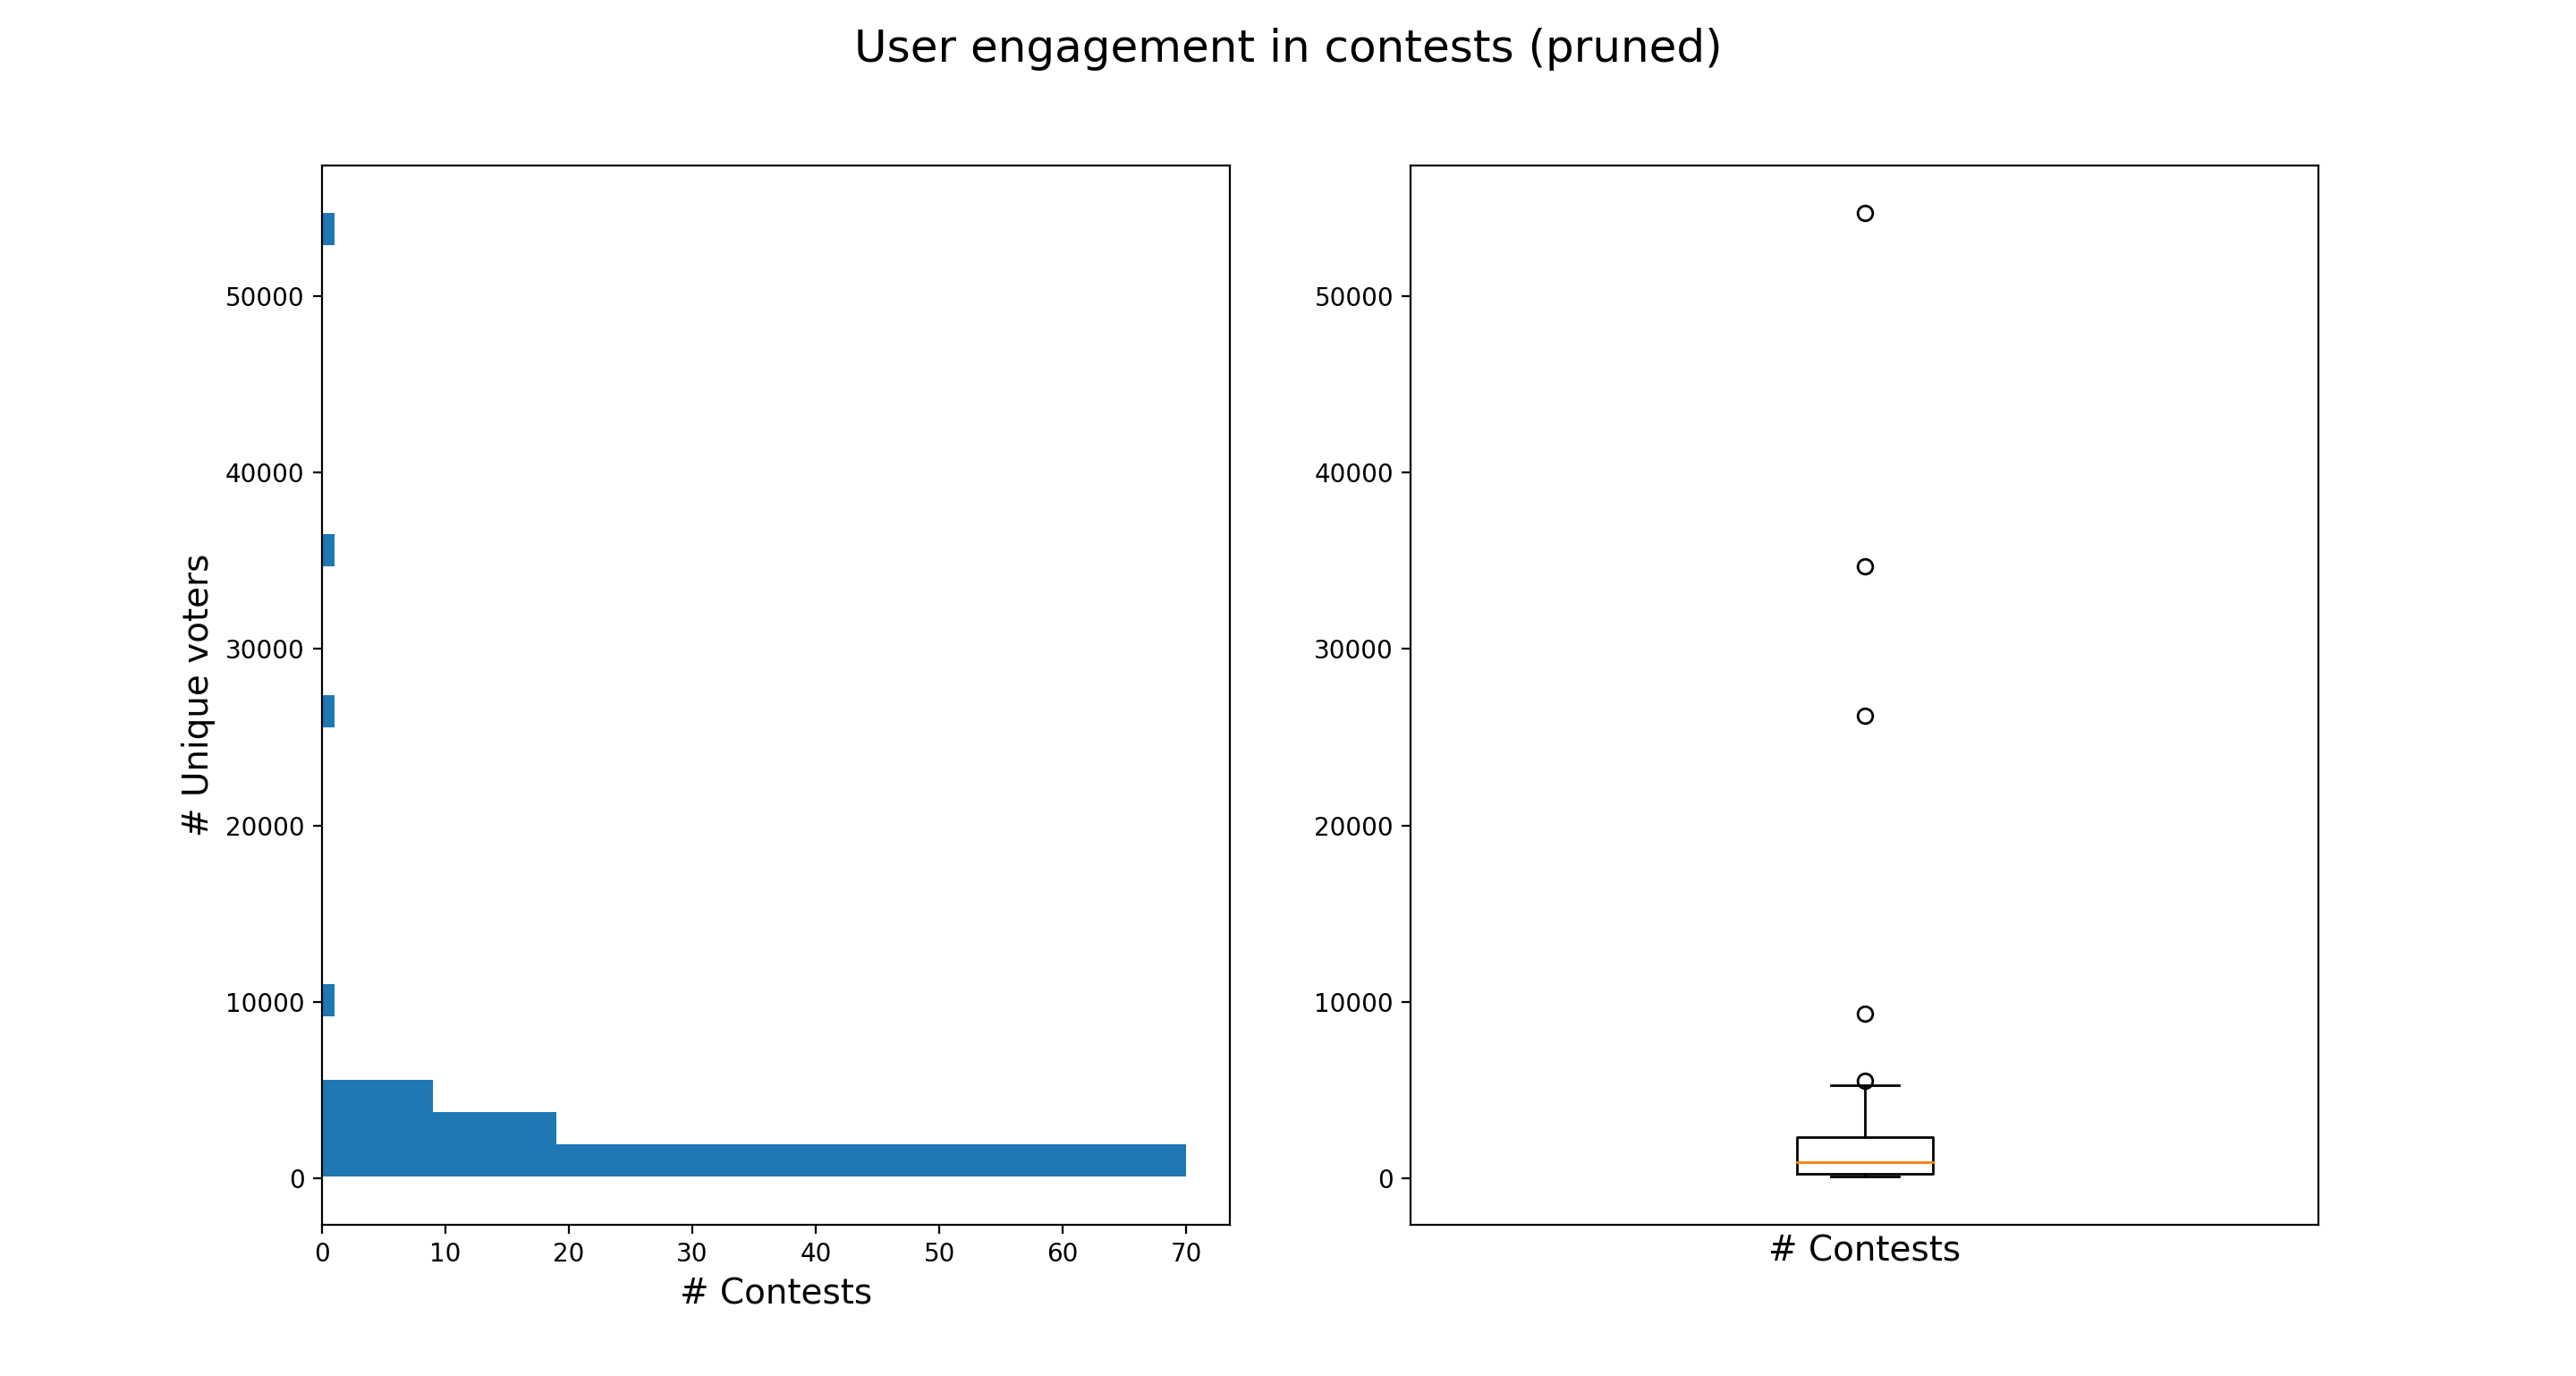
\includegraphics[width=0.8\textwidth]{Images/user_engagement_in_contests-pruned.png}
            \caption{The number of unique voters over contests after filtering out contests with less than $100$ unique voters.}
            \label{user_engagement_in_contests-pruned}
        \end{center}
    \end{figure}
    
    The six large contests are worth investigating a bit more closely. Four \footnote{\url{https://choicely.com/contest/5ca98554-0f7d-11e7-9f0c-6f102a54d68d}}\footnote{\url{https://choicely.com/contest/fb112461-9000-11e6-9e28-87ebd7a21d0d}}\footnote{\url{https://choicely.com/contest/7425566e-8c8e-11e6-b8ce-2147b021362f}}\footnote{\url{https://choicely.com/contest/164f52c7-9df8-11e7-b3c9-d1a0f88250ad}}
    out of the six large contests were beauty pageants, labeled with the categories of "beauty", "fashion" and "entertainment". The two other contests
        \footnote{\url{https://choicely.com/contest/50819173-f838-11e6-b171-b949f18a4d21}}
        \footnote{\url{https://choicely.com/contest/4257ea9c-3e21-11e7-84ec-5f5a9bcfd190}}
    are listed only in the "other" category, which is certainly a mistake. By looking at the latter two contests, it can be easily seen that they would better belong to the "entertainment" and "sports" category. In each of the contests, the contest participants were people: either sportsmen, celebrities or beauty queens/kings. It is interesting that none of the large contests have had objects, places or other intangibles as contest participants, although the platform has seen many of such participants previously. The number of participant in these contests varies between $9-40$ and their correlation coefficient does not show strong relationship either way ($R = 0.53$). 

    In the next step, let us look at the distribution of contest categories in the filtered set of contests. It can be seen from the histogram on Figure \ref{contests_over_categories}, that the amount of "beauty", "entertainment", "sport" and "fashion" contests is considerably high compared to the rest of the categories. This finding is well aligned with the case company's profile at the point of conducting this study. As pointed out in Chapter \ref{section::introduction-to-the-choicely-voting-platform}, most of the company's customer base consits of Finnish broadcasters and advertisers. Hence there is no surprise in the distribution of the categories except for the "other" group. 
    
    \begin{figure}[h] 
        \begin{center}
            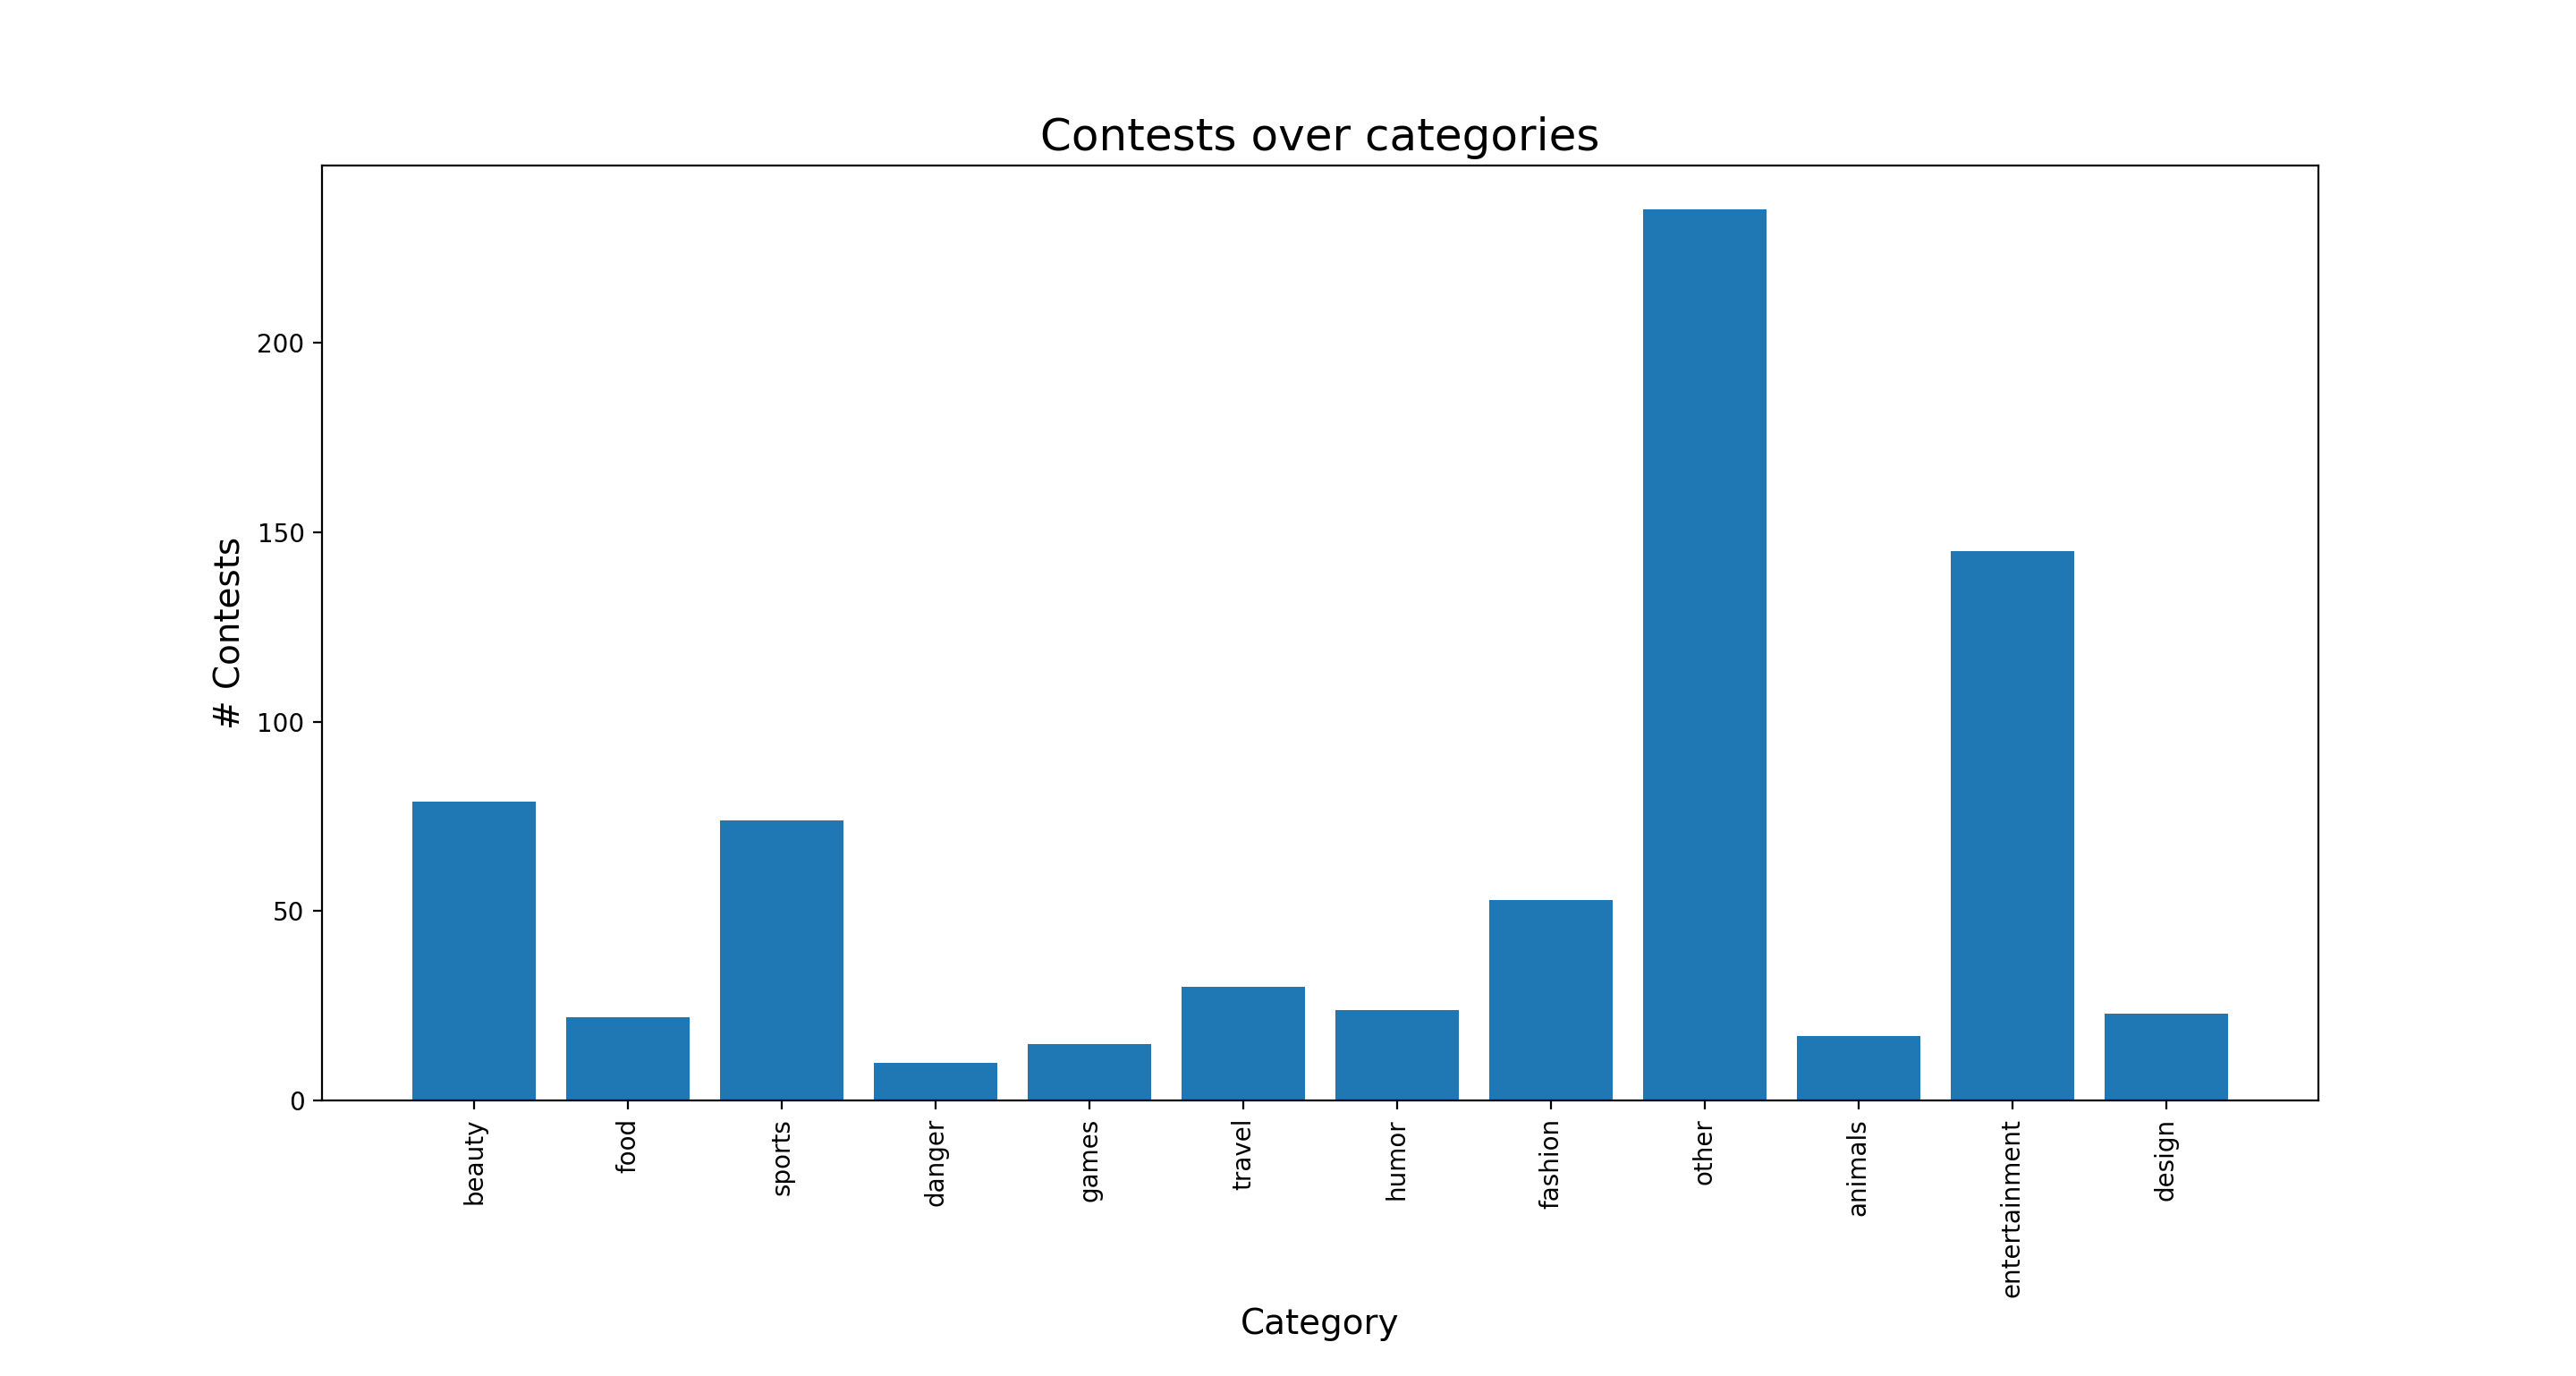
\includegraphics[width=0.8\textwidth]{Images/contests_over_categories.png}
            \caption{The number of contests in each category.}
            \label{contests_over_categories}
        \end{center}
    \end{figure}
    
    By manually looking at contests in the "other" category it can be seen, that many (28 out of 34) of these contests is actually a sport-related. To name a few examples, there are contests with titles as "Best player poll" ("Paras pelejaa aanestys")\footnote{\url{https://choicely.com/contest/5f8f8470-914d-11e6-bd5b-e571d894172f}}, "Who is the hottest driver?" ("Kuka on kuumin kuski?")\footnote{\url{https://choicely.com/contest/93d5f89c-5676-11e7-8cf7-0759c198269e}}, "Fastest driver of the race" ("Kisan nopein kuski")\footnote{\url{https://choicely.com/contest/bb7db707-3683-11e7-9f48-cbe34704f83e}}. This finding is not a suprise knowing the firm's customer base, but it also suggests the popularity of sports contests. If these contests were labelled correctly, sports contest would top the charts (Figure \ref{contests_over_categories}) with the highest bin around 50. Another interesting fact is, that in all of the sports contests, participants are athlethes, hence the images contain human beings as well. 
    
    Moreover, three of the contests were related to the "travel" category, one to "fashion" and "beauty" and one to "entertainment". The error in this case is not as high as with sport contests, however correcting these category labels would facilitate data analysis in the future. For this reason, it is suggested to the company to review such issues, correct them manually and potentially prevent them happening in the future. 
    
    To answer the question of most engaging contest categories, the unique voters over contest categories is studied. Simple statistical measures (sum, mean, median and standard deviation) are calculated for the number of unique voters for each contest category. Table \ref{user_engagement_over_categories} displays the results.
    
    It can be seen, that "entertainment" and "beauty" contests cover the majority the amount of uniuqe voters ($\approx 66.60 \%$ of the total). The values of these categories together are similar with the  "fashion" category. In these categories the mean and the median of the voters is also considerably high, which suggests their attractiveness. However, the high values in the standard deviation of the unique voters indicates the wide spreadness of values around the mean. The relevance of this observation is, that not all contests in these categories engage a large audience necessarily. Thus it can be concluded, that these categories tend to appear together and also attract a larger audience compared to the rest in general. 

    \begin{table}[]
        \centering
        \begin{adjustbox}{width=1\textwidth}
            \begin{tabular}{l|c|c|c|c|c}
                \textbf{Contest category} & \textbf{Sum of unique voters} & \textbf{Mean of unique voters} & \textbf{Median of unique voters} & \textbf{Standard deviation of unique voters} \\
                \hline
                beauty & 135866 & 3996.06 & 1482.00 & 9854.14 \\
                other & 61455 & 1807.50 & 1240.50 & 1831.40 \\
                entertainment & 161233 & 5374.43 & 1728.50 & 11772.68 \\
                sports & 15220 & 634.17 & 299.00 & 757.83 \\
                fashion & 75872 & 4742.00 & 874.00 & 12972.72 \\
                travel & 4451 & 1483.67 & 409.00 & 1719.40 \\
                humor & 1367 & 683.50 & 683.50 & 274.50 \\
                food & 767 & 767.00 & 767.00 & 0.00 \\
                danger & 958 & 958.00 & 958.00 & 0.00 \\
                games & 164 & 164.00 & 164.00 & 0.00
            \end{tabular}
        \end{adjustbox}
        \caption{The basic statistical measures of unique voters for each contest category.}
        \label{user_engagement_over_categories}
    \end{table}
    
    The categories "travel", "humor", "food", "danger" and "games" have hosted only a considerably low number of contests (Figure \ref{contests_over_categories}). Due to the small amount of data, it is difficult to derive any relevant results about the attractiveness of these categories at this point. It is suggested for the company to host and advertise more of these contests so that the public's opinion and engagement can be evaluated in these areas as well.

    % As the last part of the EDA, the attributes of highly rated contestants are investigated. In other words it is studied, what kind of traits make a contest participant more attractive to users. To answer this question, the podium finishers of the six large contests explained above are taken as examples. % TODO consider if needed

    % deriving results
    The above results contribute towards answering RQ2. The results allow to derive the following conclusions: 

    \begin{itemize}
        \item many of the contests are not labeled and hence belong only to the "other" category - fixing these labels manually could contribute towards better results,
        \item the "fashion", "beauty" and "entertainment" categories often appear together in contests,
        \item contests in the "beauty" and "entertainment" categories appear to be engaging to large audiences,
        \item contests where participants are human beings appear to be attractive to users,
        \item there is no correlation between the unique voter count and the number of participants,
        \item the platform has hosted only a few contests in some of the categories and hence it is not possible to derive significant findings about the attractiveness of those contets at the moment.
    \end{itemize}

\subsection{Association analysis}
The results of the analysis are presented for the 1-itemsets and 2-itemsets in order to keep the findigs easily understandable. The following figures display the results. The itemsets in the figure are ordered by the variance in the support values (however the variances are not displayed in the figures). This way the itemset with the highest variance is on the top, while the itemset with the smallest variance is on the bottom of the figure. All of figures in this chapter follow this convention of ordering. First the chosen Miss Suomi 2017 contest is analyzed, followed by the analysis on the system-level analysis.

Figure \ref{itemset_supports-gender-Miss_Helsinki-1_itemset} displays the results for the 1-itemset supports in case of genders. The first finding to note in this figure are the bottommost \textit{\{"beauty"\}} and \textit{\{"dress"\}} itemsets with support values 1.0 for all genders. The reason behind this observation is that all of the participants' images had these labels. Therefore, inevitably all of the vote transactions picked up these itemsets and every vote in the contest has full support towards them. Such values do not show any significant meaning and therefore are excluded from the rest of the figures.

\begin{figure}[h] 
    \begin{center}
        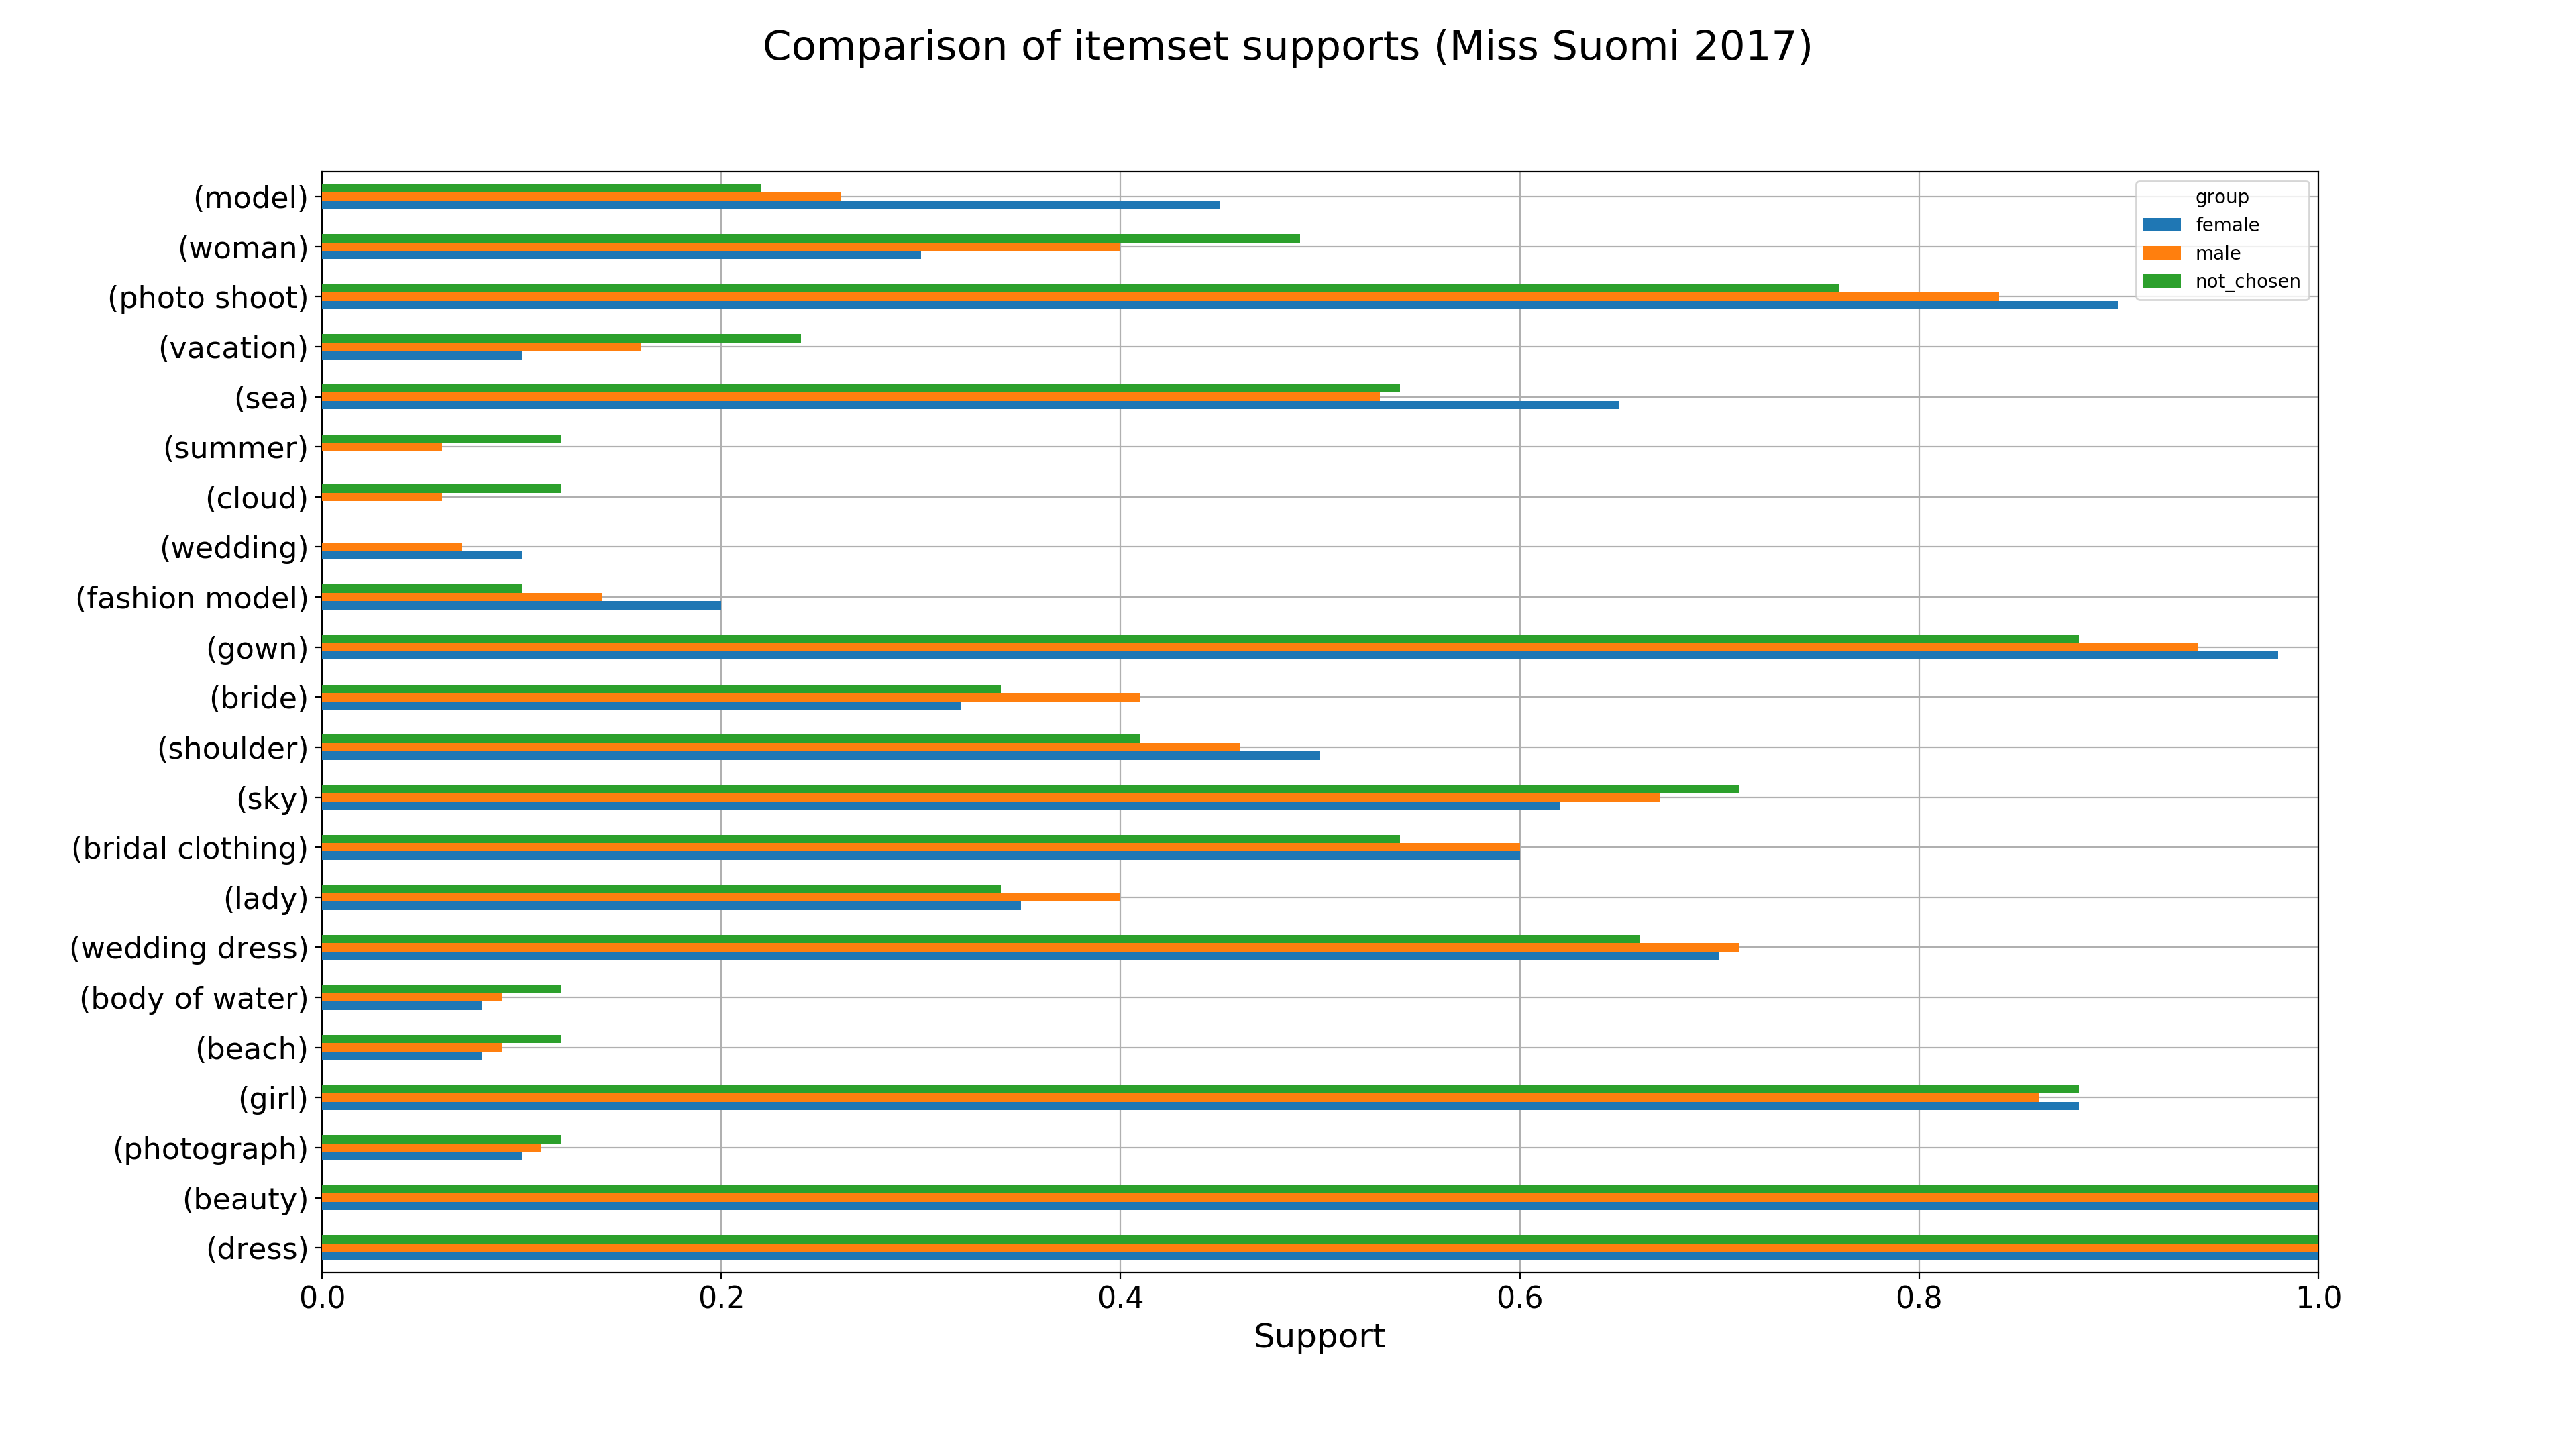
\includegraphics[width=1.0\textwidth]{Images/itemset_supports-gender-Miss_Helsinki-1_itemset.png}
        \caption{The 1-itemset supports in the Miss Suomi 2016 contest by genders.}
        \label{itemset_supports-gender-Miss_Helsinki-1_itemset}
    \end{center}
\end{figure}

It is interesting to investigate, why all of the images contained these two labels in general. As the participants' images were shot in a similar environment, with considerably similar content (e.g. the white dresses, the hair style, only one model in the image etc.), the Google Vision API assigned the same labels to the images. This gives a proof that computer vision in this case is more targeted towards getting an overall idea about the content of an image, rather than identifying its specific traits and attributes. It would be interesting to assign labels or tags manually on top of the computer's labels and compare results of a similar analysis.

This visualization provides a good possibility also to compare gender differences. For instance, the support $S(X=\{"model"\}|gender=female)=0.45$ is considerably high than its male counterpart (0.26). Similar observations can be made in case of the \textit{\{"photo\:shoot\}, \{"sea"\}, \{"gown"\}, \{"fashion model"\}} and \textit{\{"wedding"\}} itemsets. This may suggest that females are more likely to vote on images, where the object (the model and the dress) is put more into focus. Interestingly, the support for the \textit{\{"cloud"\}} and \textit{\{"summer"\}} itemsets are 0.0 for females and are higher for males. This means that no female users have voted on images with these labels (unless they belong to the \textit{not\_chosen} gender). This allows the conclusion that males might prefer images with more light and more colorful background in their votes. The support for \textit{\{"bride"\}} and \textit{\{"lady"\}} itemsets for males are also higher, which can mean that the impact of the model being a girl has more impact on their votes than her dress or the surroundings.

Figure \ref{itemset_supports-age_group-Miss_Helsinki-1_itemset} shows the 1-itemset supports for age groups. It is interesting to notice that age groups 45-54 and 65+ have considerably higher values than the rest of the groups in case of the \textit{\{"bridal clothing"\}}, \textit{\{"gown"\}} and the \textit{\{"wedding dress"\}} itemsets. In other words it appears, that the clothing displayed on the pictures is more engaging for these groups. This may indicate that that dresses that appear on the images become influental in favouring a model in this kind of a contest. 

\begin{figure}[h] 
    \begin{center}
        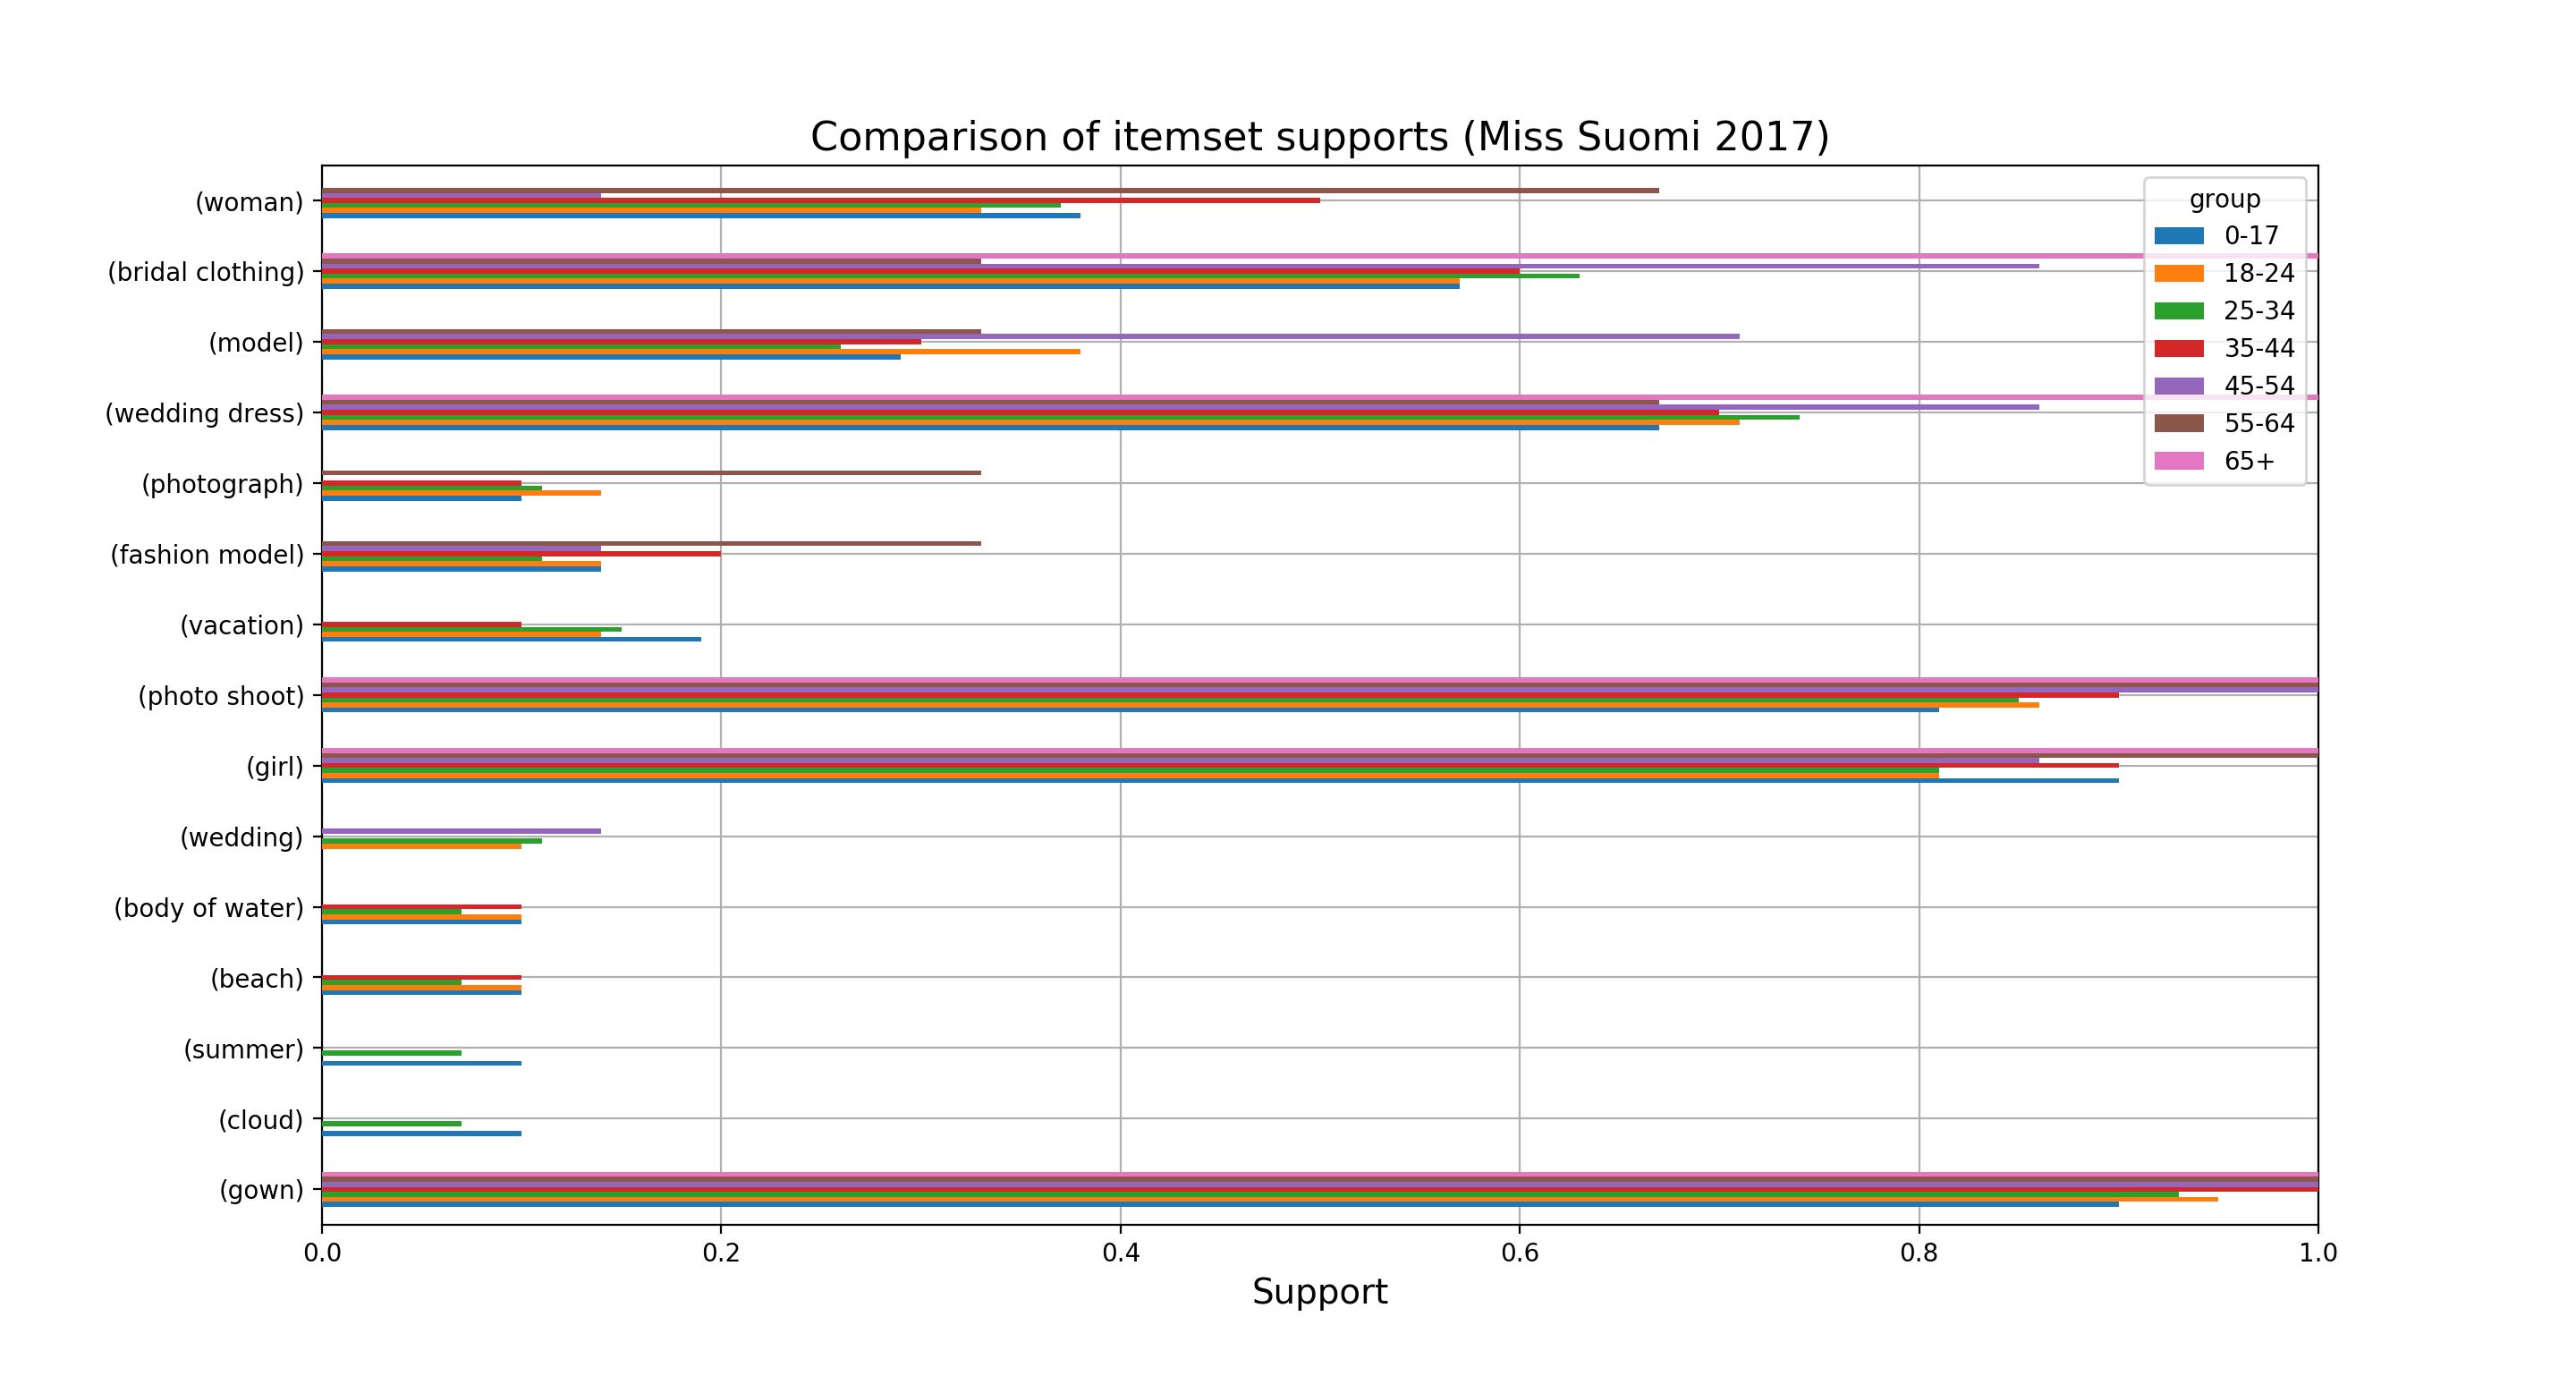
\includegraphics[width=1.0\textwidth]{Images/itemset_supports-age_group-Miss_Helsinki-1_itemset.png}
        \caption{The 1-itemset supports in the Miss Suomi 2016 contest by age groups (first 15 only).}
        \label{itemset_supports-age_group-Miss_Helsinki-1_itemset}
    \end{center}
\end{figure}

Another interesting observation is that the support for some itemsets, such as \textit{\{"body\:of\:water"\}, \{"beach"\}, \{"cloud"\}, \{"vacation"\}, \{"beach"\}} show 0.0 support for the groups above age of 45. At the same time, these itemsets show somewhat higher support by the age groups on the lower end. This finding may indicate that activities such as having vacation on a beach in a warm country is more in the interest of young people, which can be valuable information for travel agencies or marketing specialists. With such valuable informations at hand, tourism offices could provide more customized advisory service for customers with different background. 

Finally, the 1-itemsets supports in the contest are analyzed by the location (country) of the users (Figure \ref{itemset_supports-country-Miss_Helsinki-1_itemset}). The first interesting observation is, that the support of the USA group is $1.0$ on some itemsets, while 0.0 on the others and there are no values in between.

\begin{figure}[h] 
    \begin{center}
        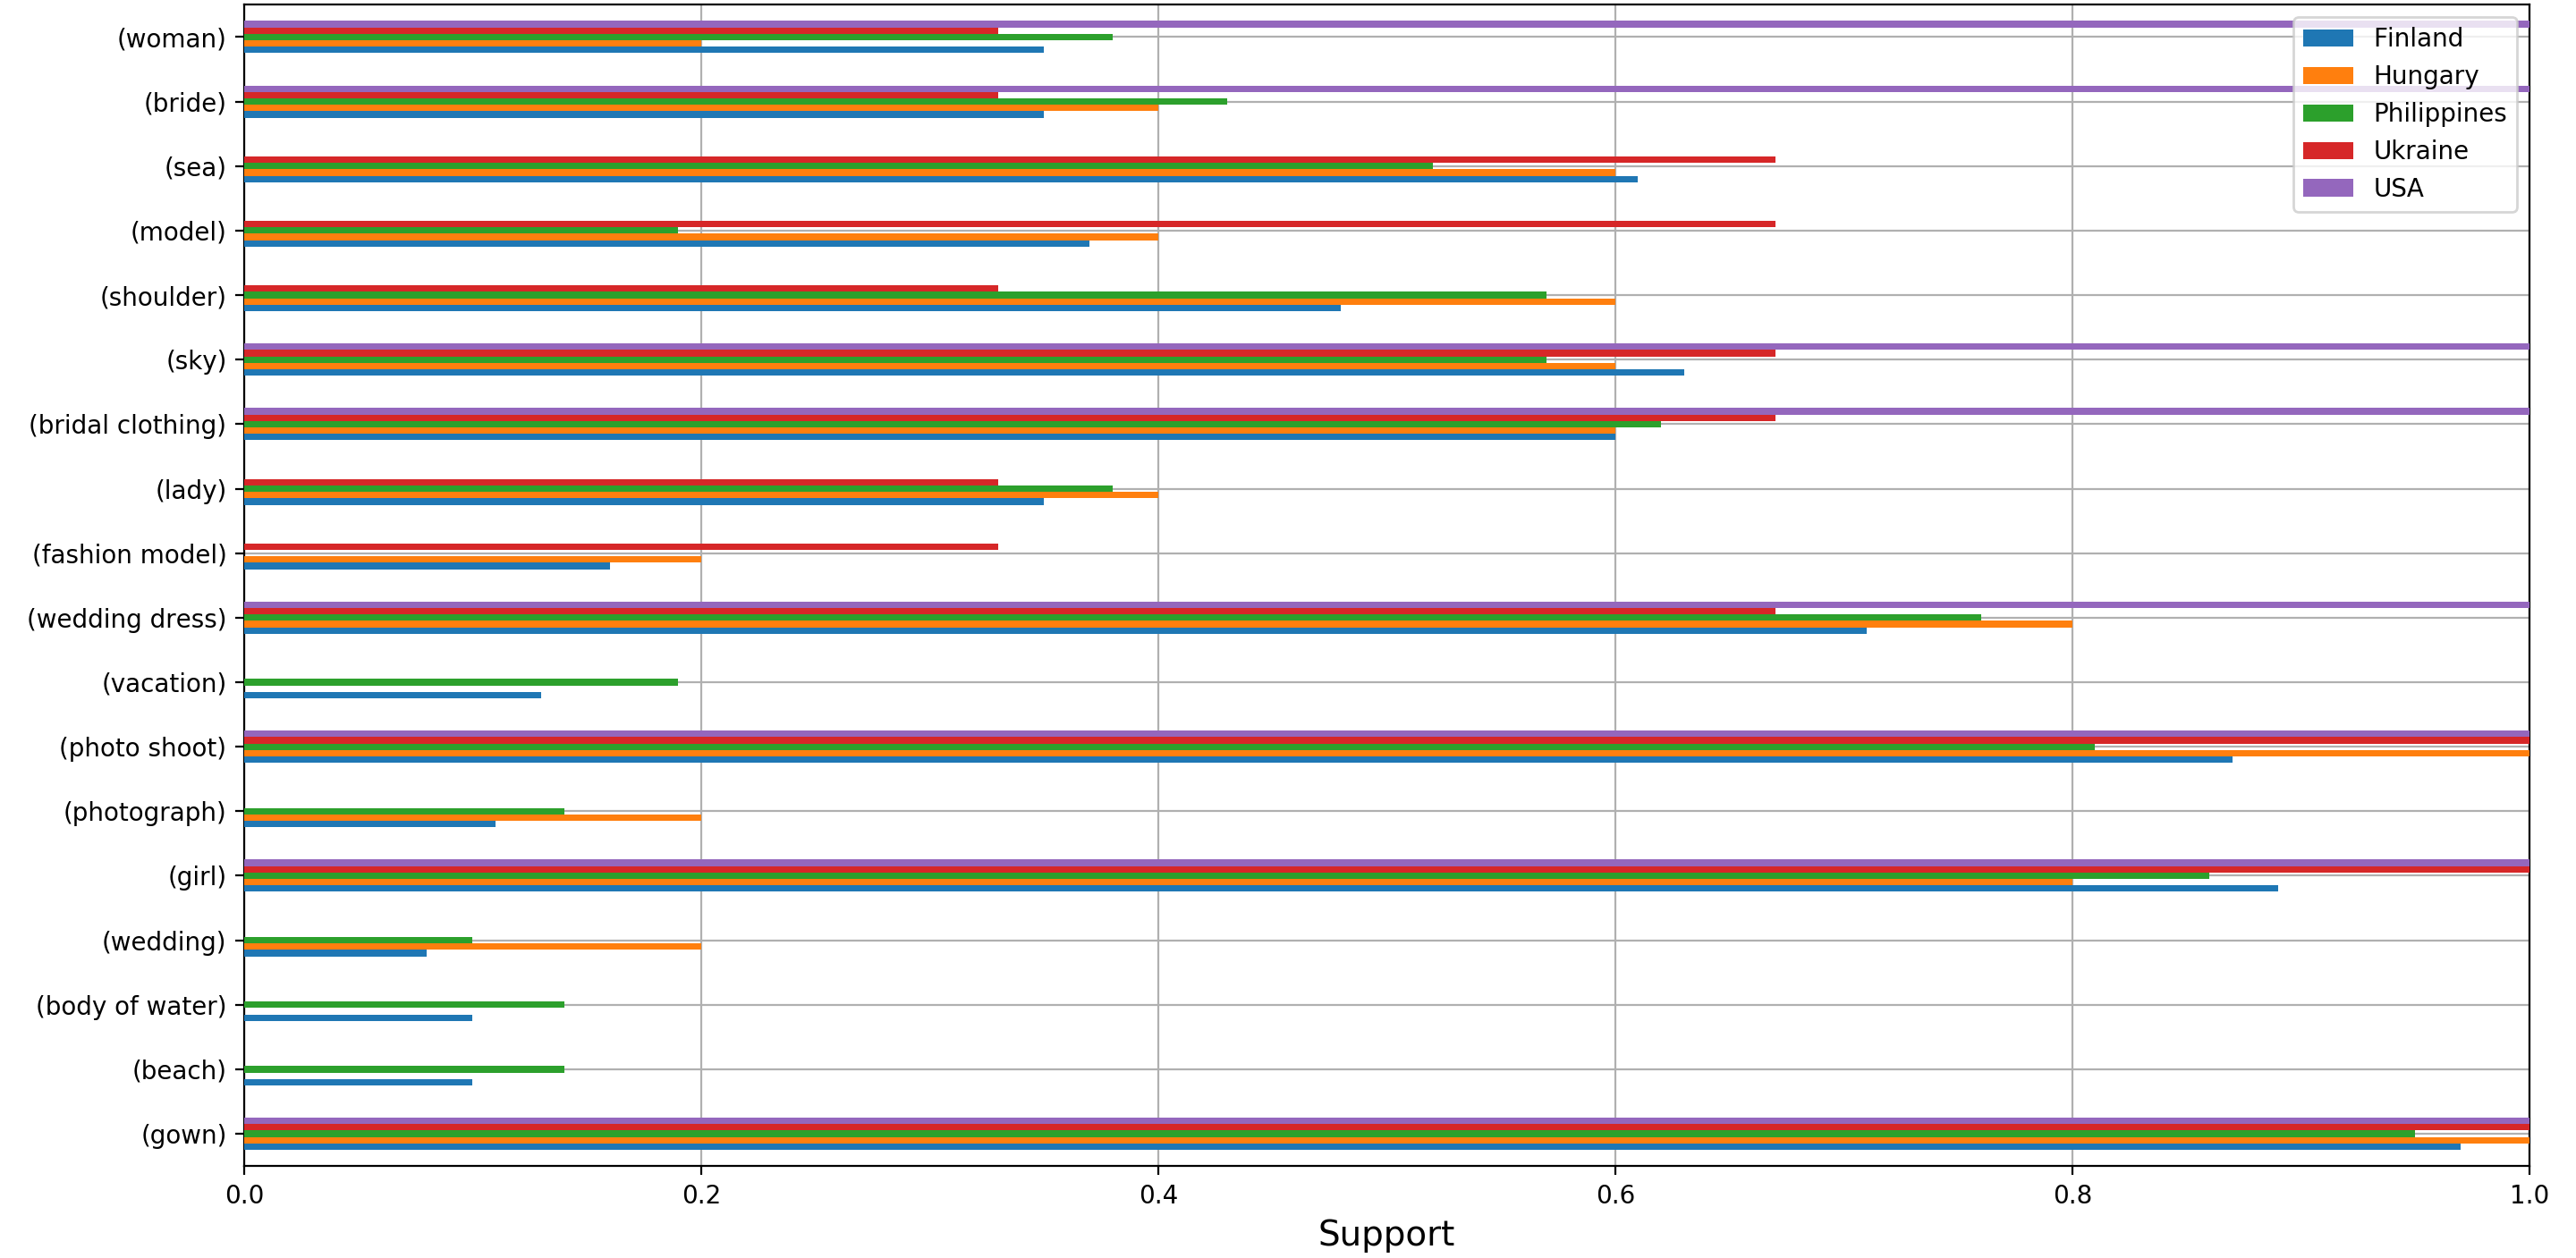
\includegraphics[width=1.0\textwidth]{Images/itemset_supports-country-Miss_Helsinki-1_itemset.png}
        \caption{The 1-itemset supports in the Miss Suomi 2016 contest by countries.}
        \label{itemset_supports-country-Miss_Helsinki-1_itemset}
    \end{center}
\end{figure}

By looking at the data the reason becomes obvious: the amount of transactions, where the users' country information is set as USA, Ukraine and Hungary are considerably low (below 5). This may not be a big surprise knowing that this contest was mainly advertised in Finland and not in other countries. As a matter of fact, there were $62$ Finnish voters and $21$ voters from the Philippines, which are still considerably low compared to the total number of voters. This finding suggests that many of the voters in this contest did not indicate their country information and hence do not display on Figure \ref{itemset_supports-country-Miss_Helsinki-1_itemset}. In other words, the amount of users, whose location information is filled is low and hence the results can get biased. 

The data shows, that many voters in this contest did not give their location information, which limits the analysis. Encouraging the users in the future to provide more information would allow to derive valid results. At the present time, no strong conclusions can be drawn from the location data of the voters in the Miss Suomi 2017 contest. 

Figure \ref{itemset_supports-gender-Miss_Helsinki-2_itemset} displays the support values for the 2-itemsets. To enhance the readability of the figure, only the first 15 values are shown. It can be seen from the figure that some itemsets have small, while some others have high support values. It can be seen that the itemsets with higher values, such as \textit{\{"girl, "wedding\:dress"\}, \{"girl", "dress"\}, \{"girl", "beauty"\}, \{"sky", "gown"\}} tend to also tell something more about the object of the image over the background. These itemsets also might stand out, because they appear often on the images. However, the data reveals that the abstract concepts (such as vacation or wedding) appear with less support. 

\begin{figure}[h] 
    \begin{center}
        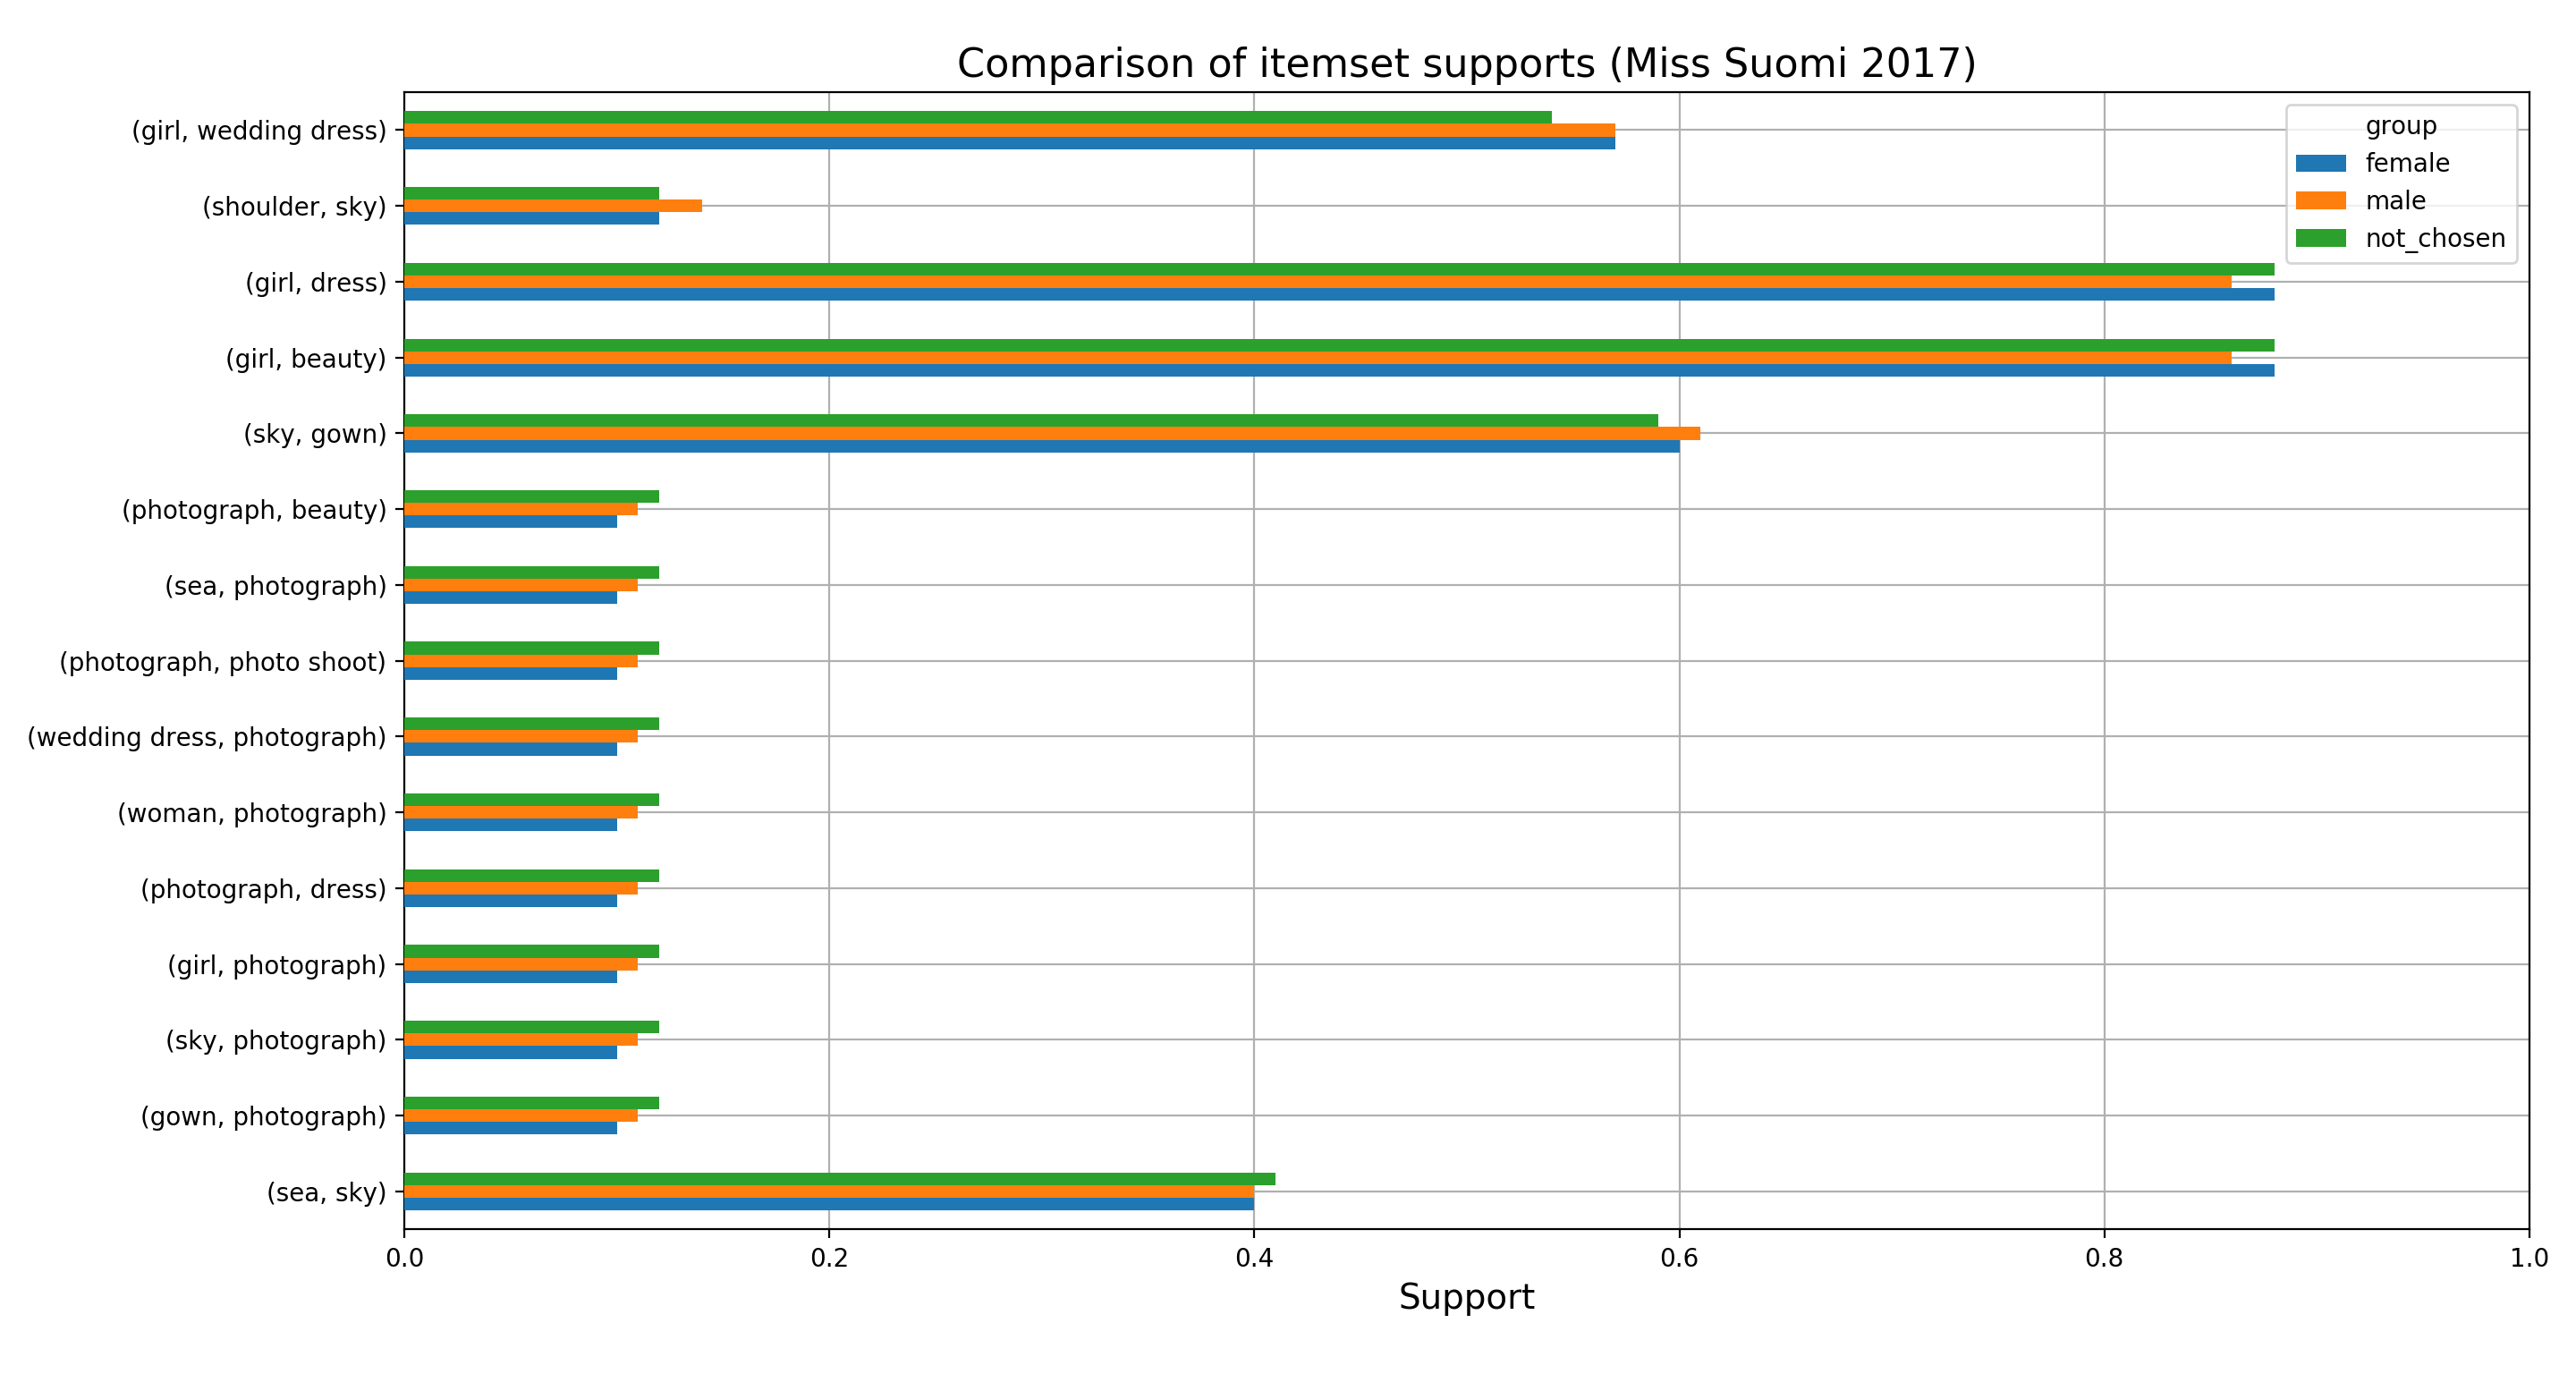
\includegraphics[width=1.0\textwidth]{Images/itemset_supports-gender-Miss_Helsinki-2_itemset.png}
        \caption{The 2-itemset supports in the Miss Suomi 2016 contest by genders (only the first 15 itemsets are displayed ordered by variance).}
        \label{itemset_supports-gender-Miss_Helsinki-2_itemset}
    \end{center}
\end{figure}

There is a total number of 150 2-itemsets in the image labels of the Miss Suomi contest, which is hard to analyze for the human eye. This number grows further with number of items in the set. To tackle this problem, itemsets with more than 1 item are not investigated the same way. Instead, the Co-Clustering approach is applied on the data to identify itemsets, that appear similar to eachother in their support. The details on this analysis are explained in this chapter. The results are presented in the next chapter.

The second part of the Association Analysis studies the itemset supports on the system level. The paragraphs to follow are dedicated to explain the findings, when this method is applied to a larger set of vote transactions composed from contests, which have engaged over $100$ unique voters. This is the same dataset, which was used for the major part of the EDA in Chapter \ref{section::exploratory-data-analysis}.

On the figures to follow the itemsets are ordered by the sum of the supports instead of their variance. This way the itemsets that have the highest overall support among demographic groups are extracted.

The results are shown on the figures below by gender (Figure \ref{itemset_supports-gender-all_contests-1_itemset}) for the 1-itemsets. The itemsets on the left side of the figure reflect on the great majority of "beauty" and "fashion" contests, as it was shown on Figure \ref{contests_over_categories} in Chapter \ref{section::exploratory-data-analysis}. It can be easily seen that all of the itemsets were extracted from contests of these two category, as they clearly describe concepts that appear in such contests. This observation also supports the previous finding, that mainly contests in these categories were hosted in the platform with great success.

\begin{figure}[h] 
    \begin{center}
        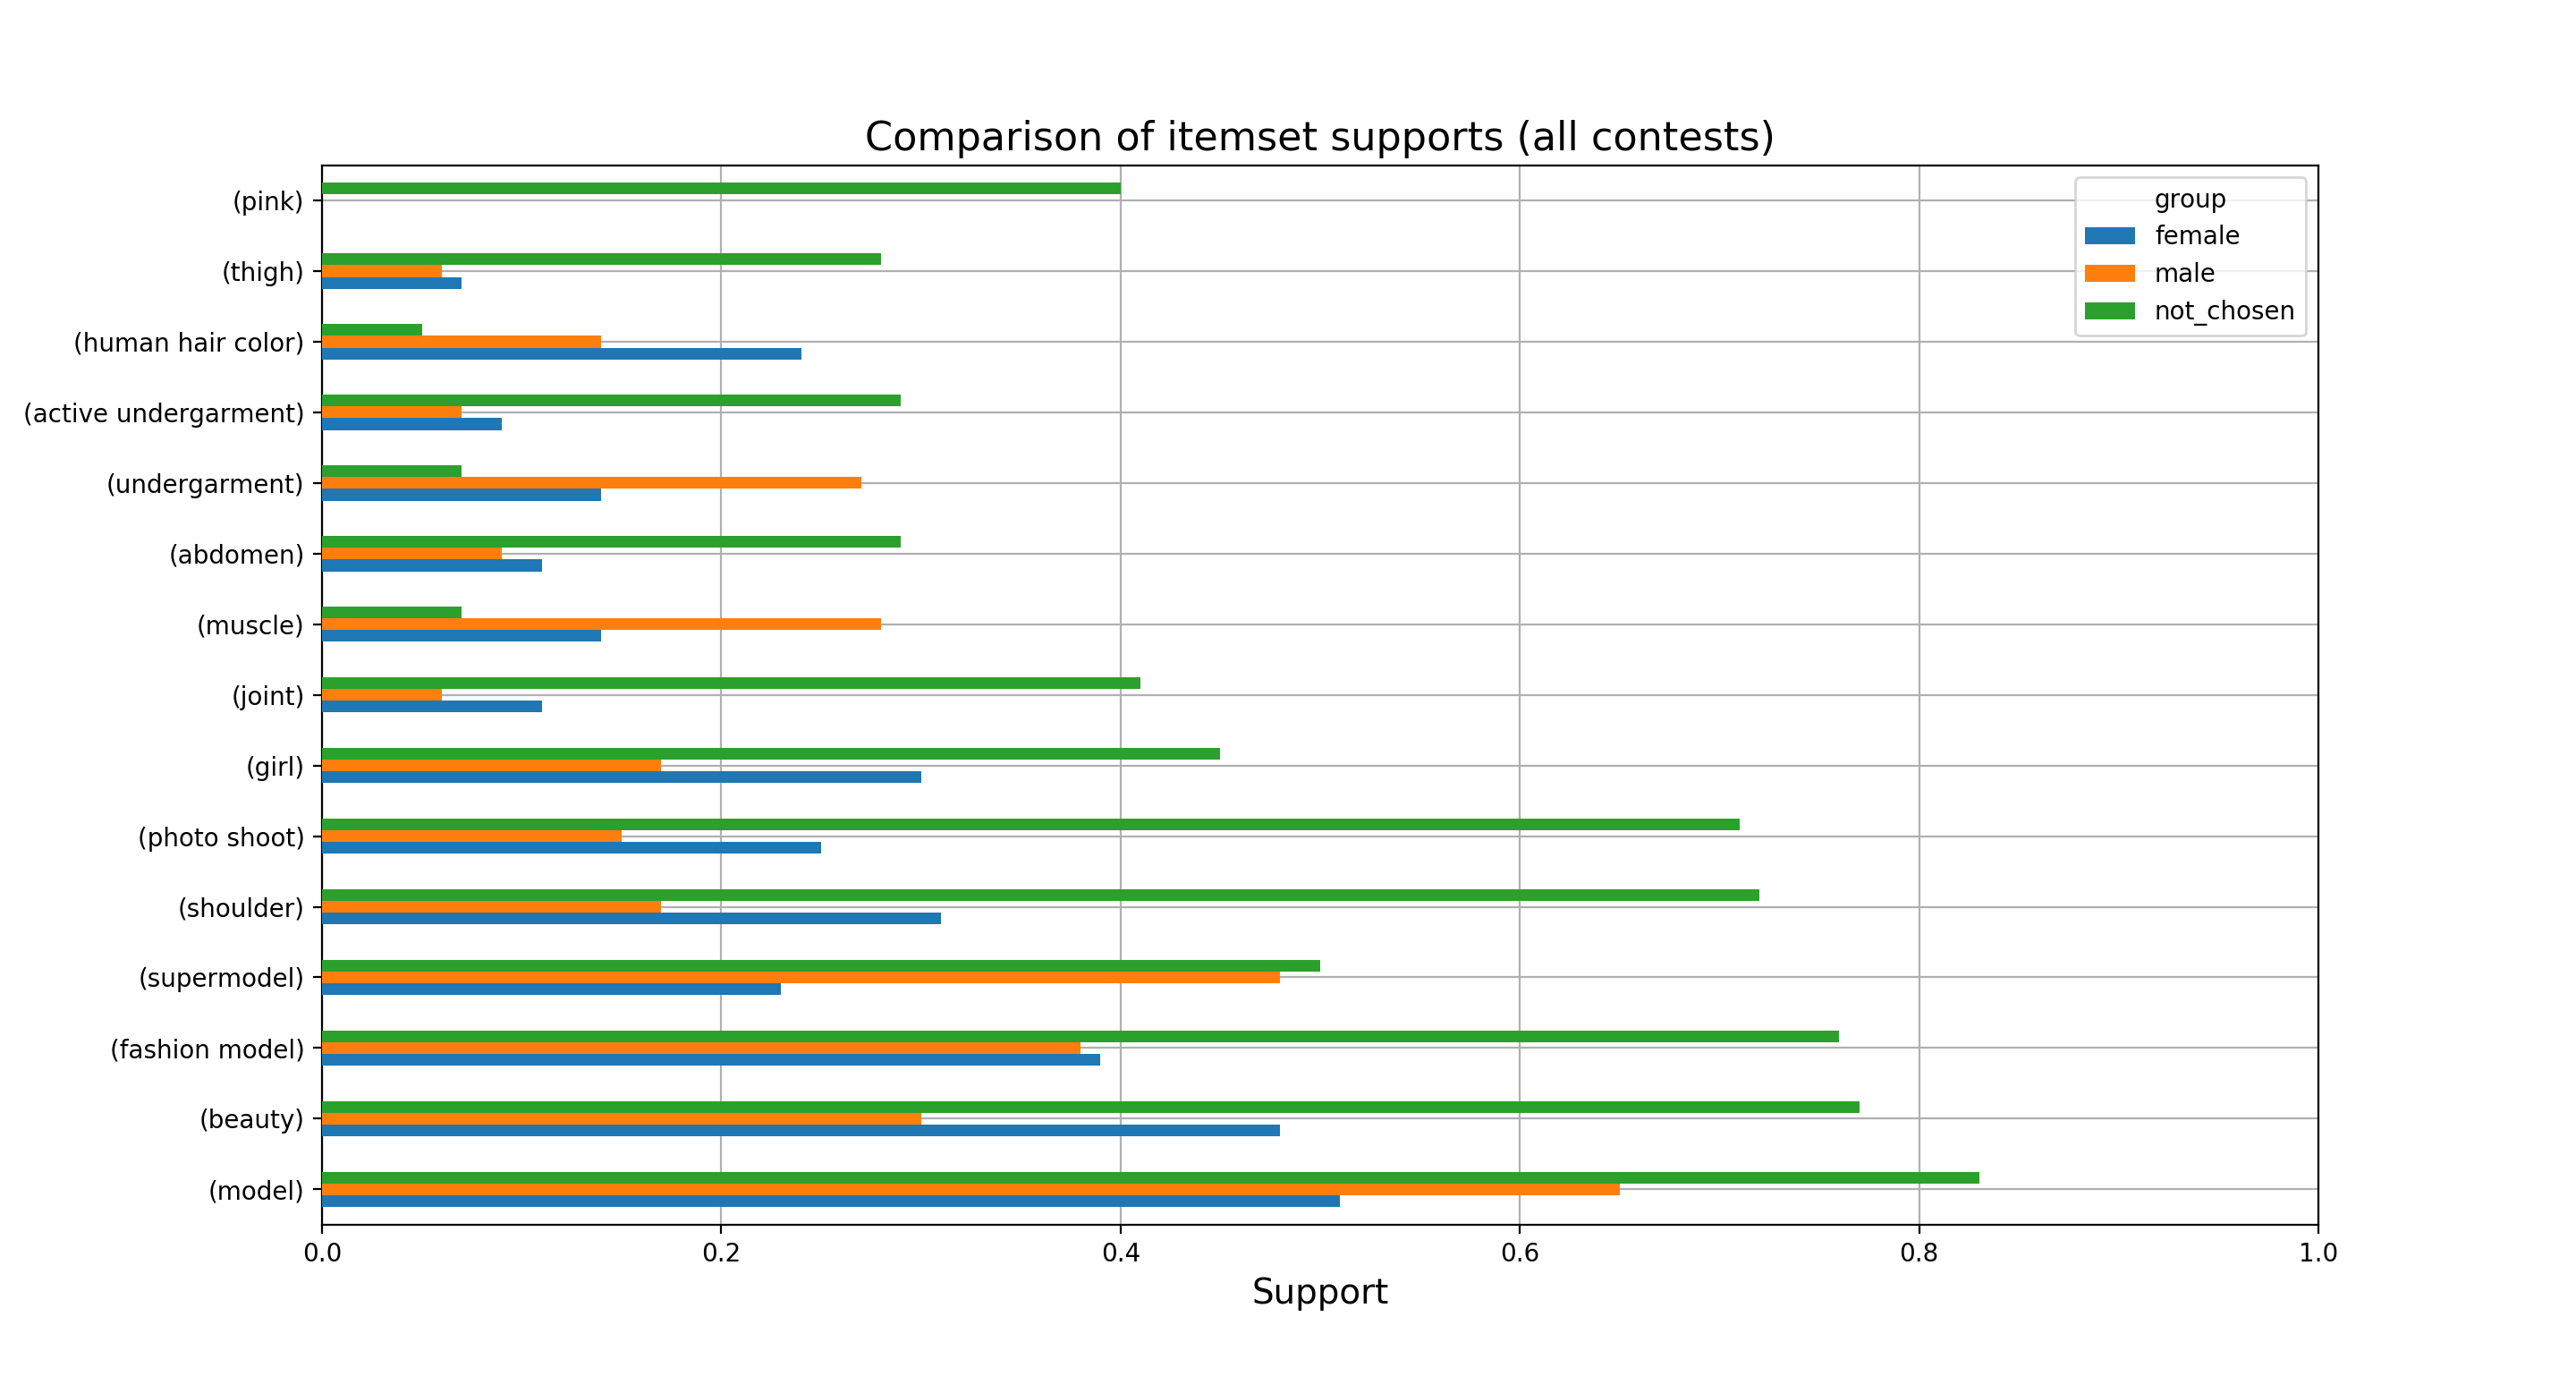
\includegraphics[width=1.0\textwidth]{Images/itemset_supports-gender-all_contests-1_itemset.png}
        \caption{The 1-itemset supports in all contests by genders (only the first 15 itemsets are displayed ordered by sum of the support values).}
        \label{itemset_supports-gender-all_contests-1_itemset}
    \end{center}
\end{figure}

Gender differences can be analyzed for the 1-itemsets on the system-level as well. For instance, males appear to have higher support towards the labels \textit{\{"model"\}, \{"supermodel"\}} and \textit{\{"muscle"\}}. This can mean that males tend to prefer contestants more with these traits even in multiple contests. Likewise, female voters have higher support value towards \textit{\{"human\:hair\:color"\}, \{"girl"\}, \{"shoulder"\}} and \textit{\{"beauty"\}}, which can mean that for them the aesthetic and potentially artistic appearence of the contender is appreciated more. 

It is interesting to observe, that the \textit{not\_chosen} group has considerably higher support over males and females in many cases. This can be explained by the fact that many users (49.82 \%) did not proide their gender information. Because the amount of such users, whose gender is not known is about the same as male and female users together in the platform, the support of this group towards itemsets appear higher. While this problem did not emerge on a single-contest level, when looking at all transactions, it becomes apparent. It could be assumed, that the distribution of the two genders is equal in this group, however there is no proof on this claim. 

Finally, all of the itemsets with more than 2 items are extracted from the system. The aim here is to identify itemsets with high support in pairs, which correspond to higher attractiveness when they appear on images together. Figure \ref{itemset_supports-gender-all_contests-over2_itemset} displays the results. It can be seen, that many of the itemsets are highly supported by the \textit{not\_chosen} user group. The reasons behind this are explained above, nevertheless the tendencies towards attractive itemsets can be observed based on this data as well. It can be seen that the \textit{"{model}"} and the \textit{"{shoulder}"} 1-itemsets often appears as a subset of various itemsets. Furthermore, contestants whose clothes are more revealing towards skin and upper body are more attractive to users. Similarly to previous findings, rather than describing the background, the itemsets on the system level are also more focused on the object of the images. 

\begin{figure}[h] 
    \begin{center}
        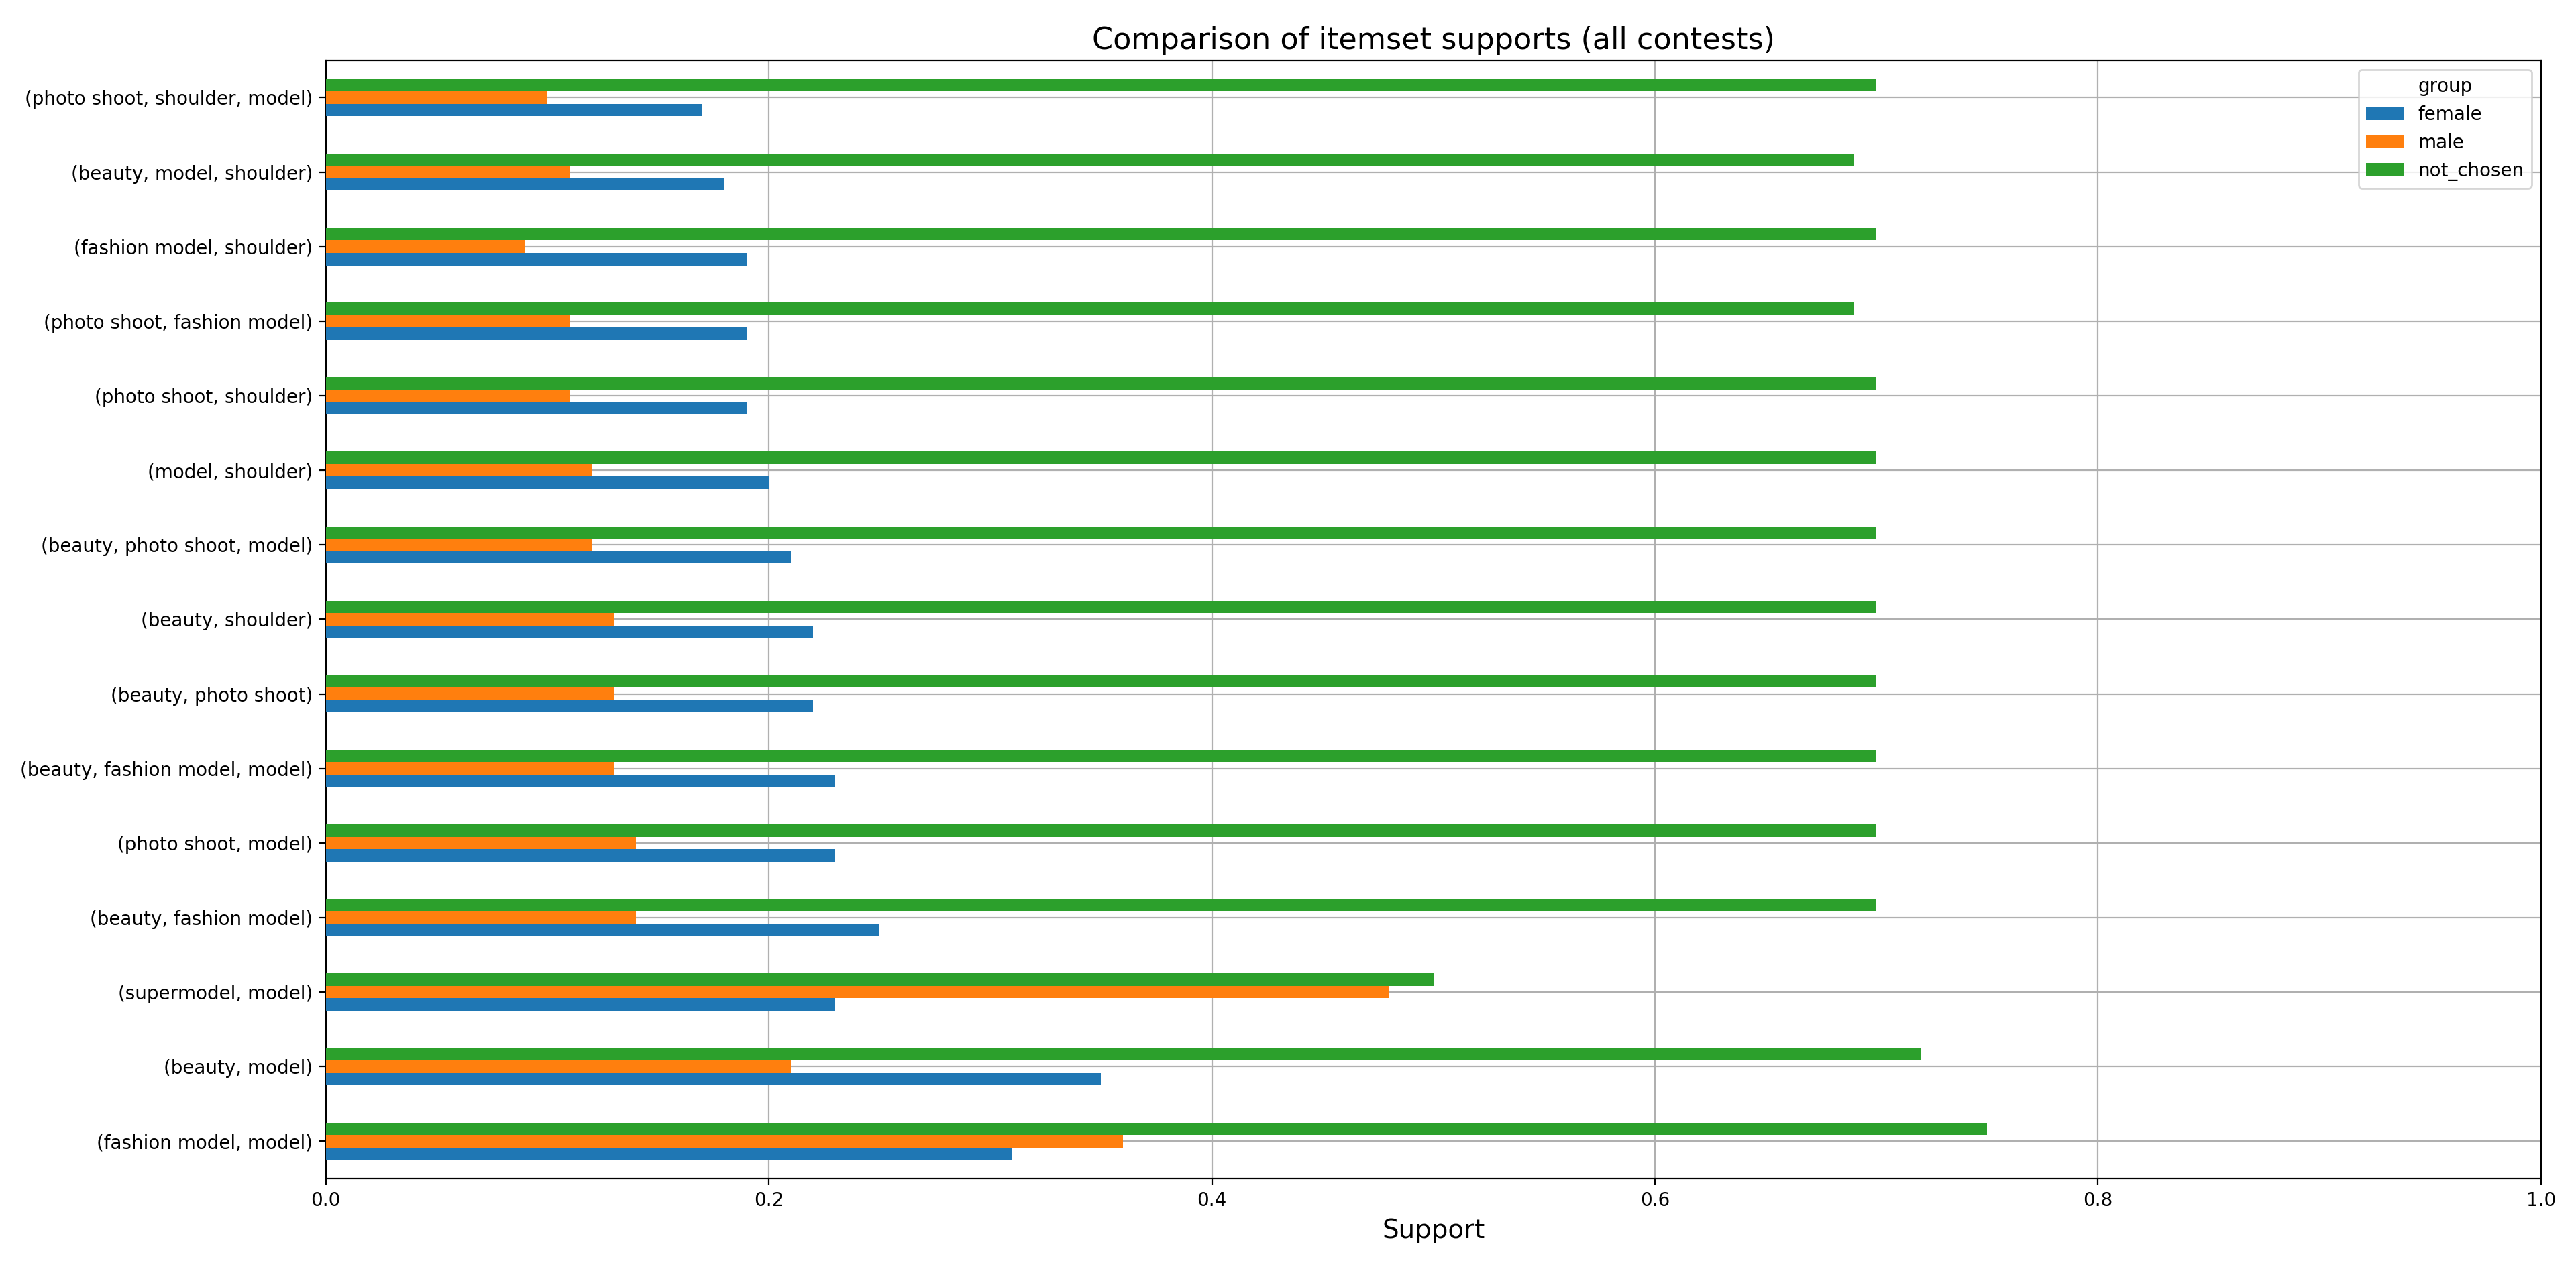
\includegraphics[width=1.0\textwidth]{Images/itemset_supports-gender-all_contests-over2_itemset.png}
        \caption{The k-itemset supports in all contests by genders, where $k \geq 2$ (only the first 15 itemsets are displayed ordered by sum of the support values).}
        \label{itemset_supports-gender-all_contests-over2_itemset}
    \end{center}
\end{figure}

\subsection{Co-Clustering}
The chosen Co-Clustering algorithm (Chapter \ref{section::methodology}) first was executed on a smaller set of 2-itemsets in the Miss Suomi 2017 contest. In this analysis, the $minsup$ value was set to $0.4$ to focus only on the itemsets with higher support. This was done in order to first understand and demonstrate how the algorithm works in a smaller scale, similarly as it was done in the previous chapters. Then the method was applied on the Miss Suomi 2017 contest as well as on the system level for all itemset sizes in both cases with the $minsup$ value of $0.05$. Various number of clusters was tried out with various observations depending on the dataset size and the demographic groups being analyzed. The results are explained in the paragraphs to follow. 

First, a smaller set of itemsets in the Miss Suomi 2017 are chosen for a more careful analysis. The filtering by support here is done by first collecting the support values of the 2-itemsets for genders and age groups (same way it was done during the Association Analysis, shown on Figure \ref{itemset_supports-gender-Miss_Helsinki-2_itemset}). Then all of the itemsets were dropped, where the highest value did not exceed the $0.4$ $minsup$ threshold. This way 54 instances of 2-itemsets remain in the dataset.

Next, the matrix of the itemsets is plotted on the left side of Figure \ref{coclustering_miss-suomi-genders-2-itemsets-04_support}. The colors correspond to the support of the itemset: the lighter values indicate smaller, the darker blue colors indicate higher support values. It can be seen that for instance the \textit{\{"dress", "beauty"\}} has high, while the \textit{\{"sky", "sea"\}} considerably low support among the demographic groups. The left side of the figure is not organized in any way, hence there is no pattern in how the colors appear in the chart. 

\begin{figure}[h] 
    \begin{center}
        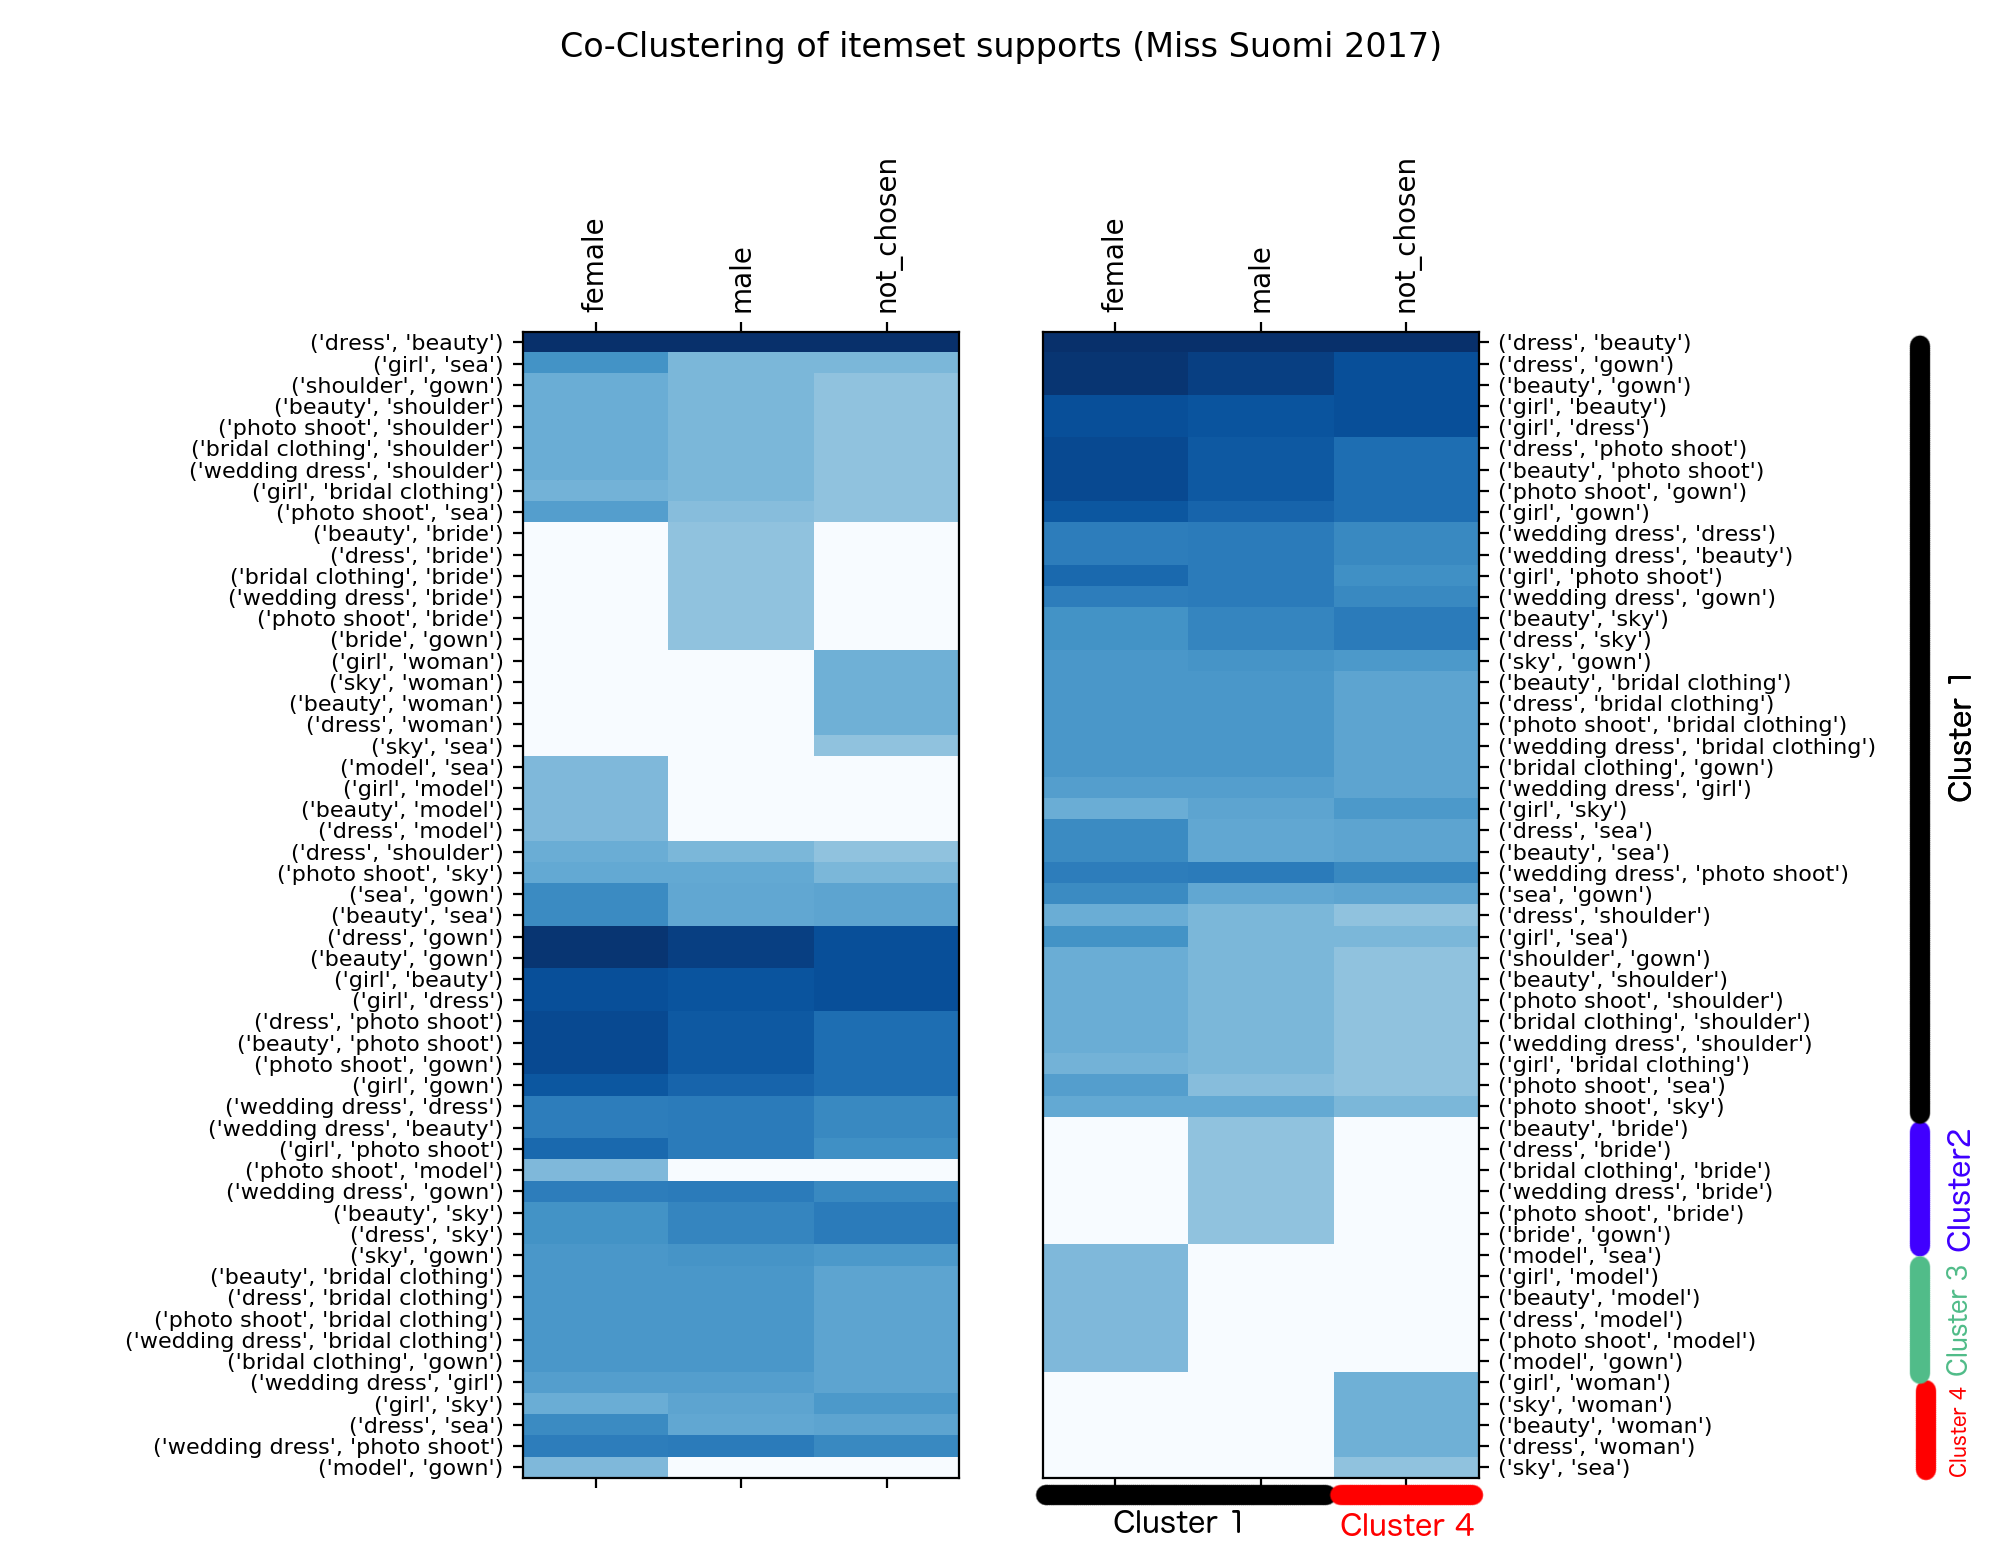
\includegraphics[width=1.0\textwidth]{Images/coclustering_miss-suomi-genders-2-itemsets-04_support.png}
        \caption{The results of the Co-Clustering in the Miss Suomi 2017 contest for 2-itemsets over 0.4 support with 4 clusters by genders. Left: the itemsets before clustering; Right: the itemsets after clustering.}
        \label{coclustering_miss-suomi-genders-2-itemsets-04_support}
    \end{center}
\end{figure}

The right side of Figure \ref{coclustering_miss-suomi-genders-2-itemsets-04_support} dislays the result of the Co-Clustering algorithm with 4 clusters. The markups on the side and the bottom of the chart indicate the clusters to which the rows and columns were assigned. Choosing the number of clusters was essentialy done by looking at the results and analyzing which k-value produces the most sensible results in this particular case. 

It can be seen that males and females were assigned to the same cluster in this case (cluster 1) with most of the itemsets that have higher support values. This finding suggests that there are no significant differences between males and females in this case. Interestingly, the algorithm has put the "not\_chosen" gorup to its own cluster (cluster 4) with only a few itemsets. This result may suggest that this group is significantly different than the other two, even though it can be seen that the supports in cluster 1 are also considerably high. 

If clusters are looked at from the aspect of the itemsets, it can be concluded which ones seem to belong together. For instance, clusters 2 and 3 clearly pinpoint the itemsets that engaged only males and females respectively in this case. This can be another useful information to marketers, whose aim is to target one of these groups with certain content. Another useful aspect in this visualization is, that the itemsets with various supports can be distingoushed easily based on the color's depth. Identifying itemsets that belong together is considerably easier on the right side of the figure as the Co-Clustering algorithm puts these close to eachother. 

Figure \ref{coclustering_miss-suomi-age_group-2-itemsets-04_support} displays the results of the same analysis for age groups. When filtering the data this way, the amount of 2-itemsets rises to 76. As there are more transactions and demographic groups, the number of clusters was increased to 5 on this occasion. 

\begin{figure}[h] 
    \begin{center}
        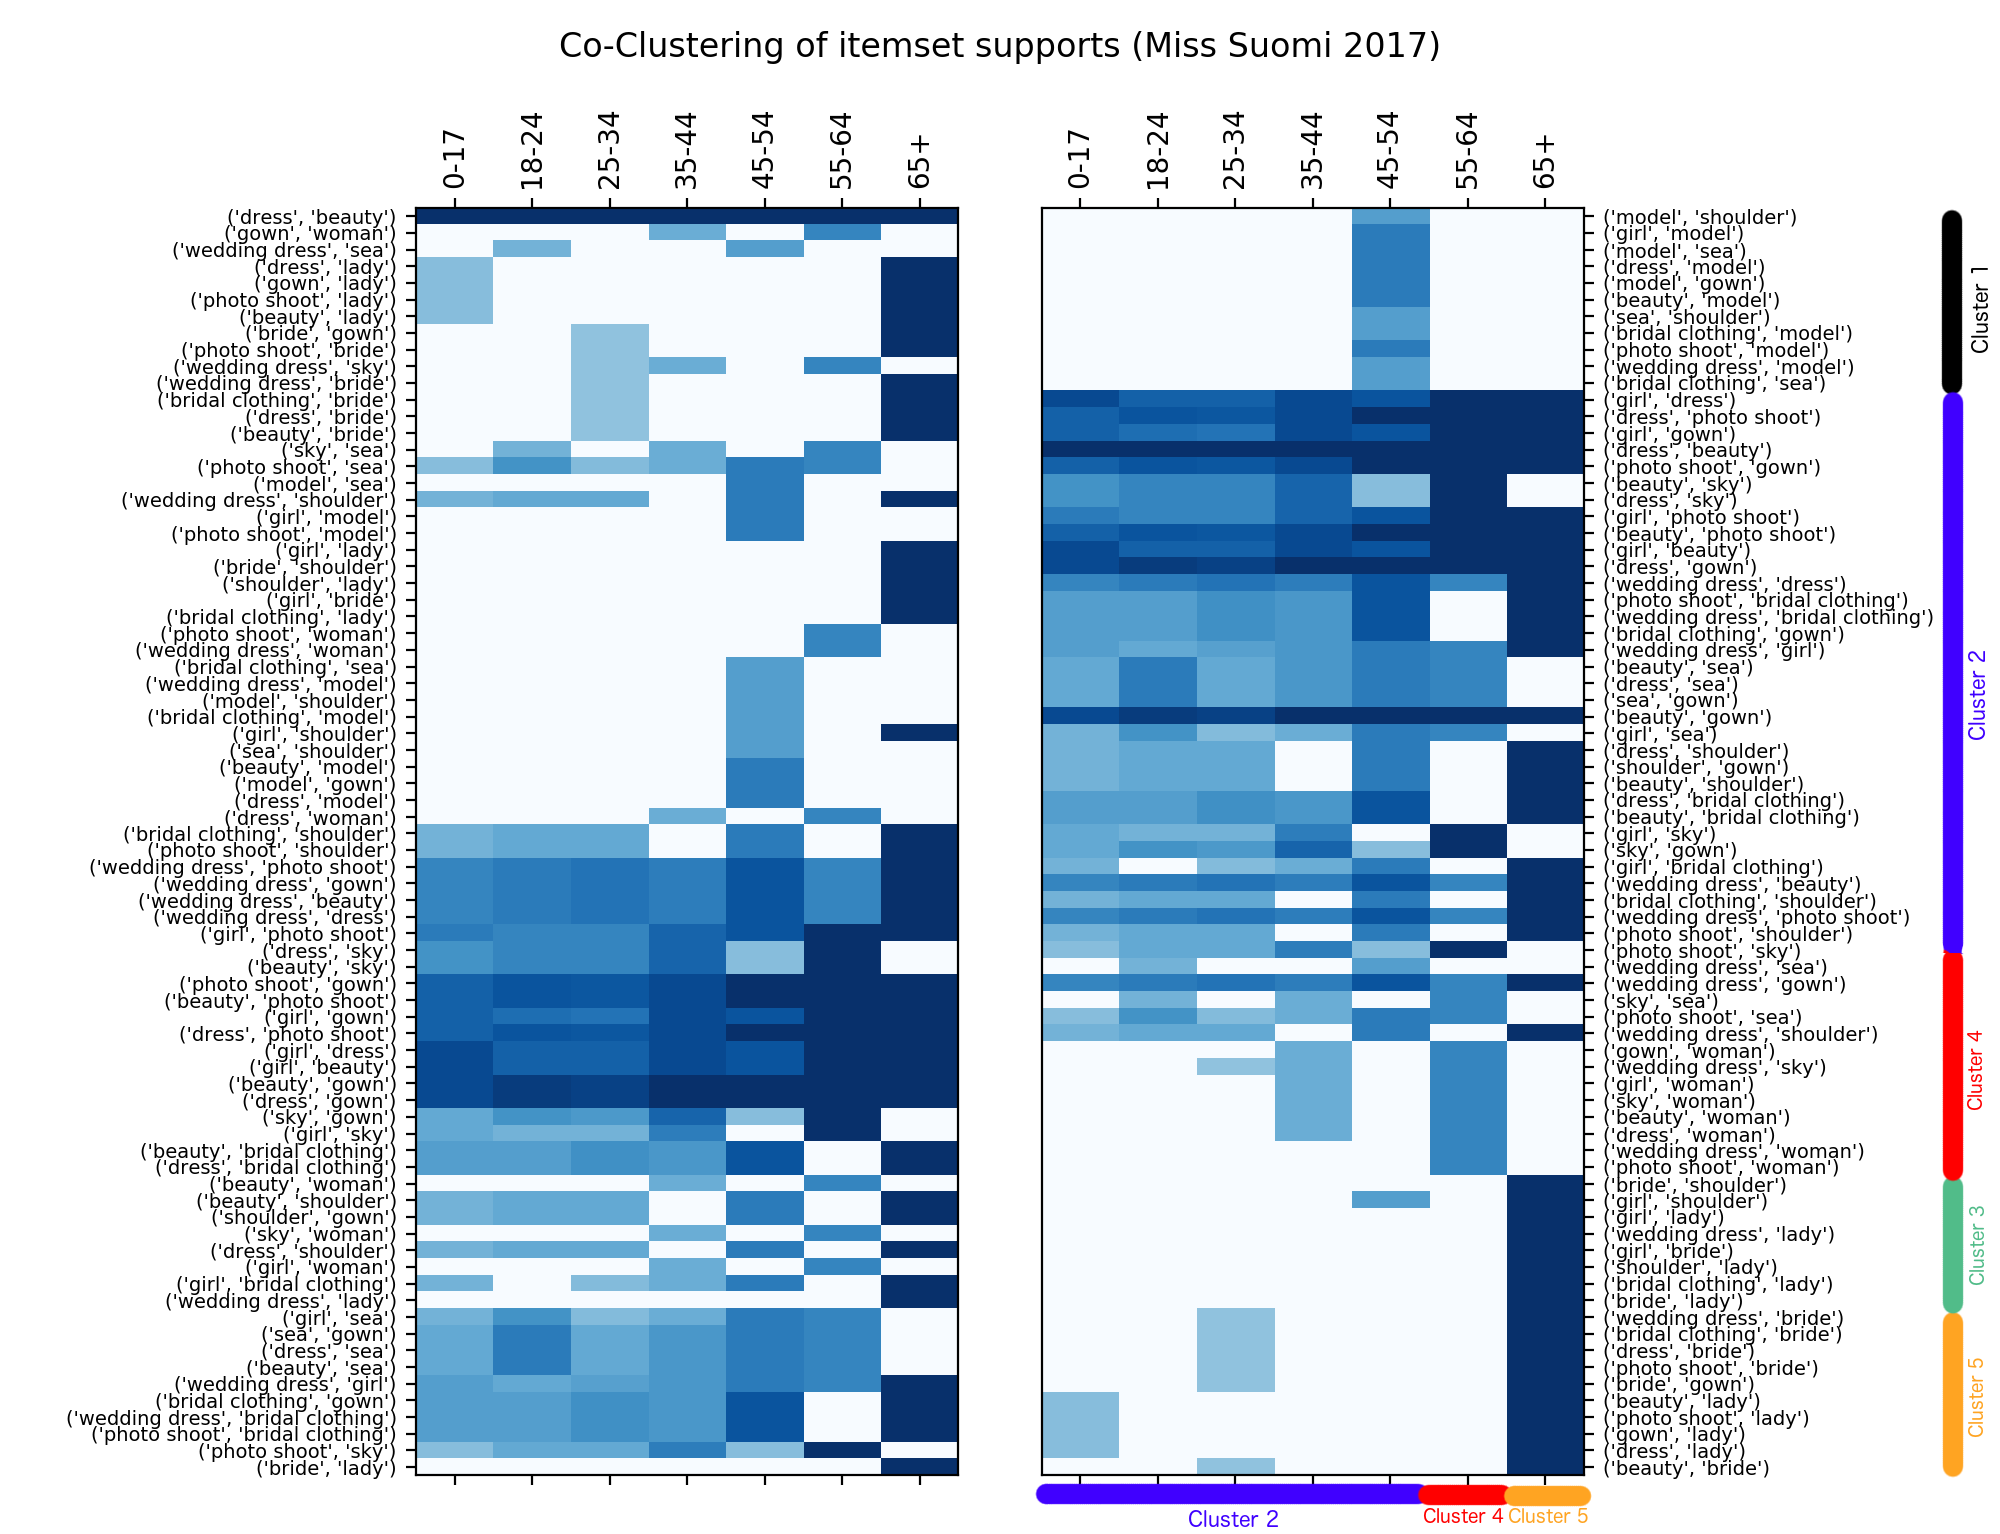
\includegraphics[width=1.0\textwidth]{Images/coclustering_miss-suomi-age_group-2-itemsets-04_support.png}
        \caption{The results of the Co-Clustering in the Miss Suomi 2017 contest for 2-itemsets over 0.4 support with 5 clusters by age groups. Left: the itemsets before clustering; Right: the itemsets after clustering.}
        \label{coclustering_miss-suomi-age_group-2-itemsets-04_support}
    \end{center}
\end{figure}

One of the most interesting observations in this case is that the age groups 45-54 and 65+ are separated from the rest of the groups. This indicates that the interests of these groups are somewhat unique compared to the others. This finding is supported by the fact that itemsets in clusters 3, 4 and 5 have higher support from one a subset of the groups. However, cluster 2 contains most of the itemsets that are supported by all of the groups. The rest of the age groups are also assigned under cluster 2, which suggests the generality of these itemsets and groups. 

It could be hence concluded, that some demographic groups follow a generalist, some others a specialist approach. In this particular case, users between the age of 0-54 are more specialists towards the itemsets in cluster 2. Likewise, users from groups 55-64 and 65+ are unique, because some content (in clusters 3, 4 and 5) is engaging only to them. As a conclusion, they could be called as generalists. This finding is in align with the results of Jang et al. \cite{jang2015no}, who also identified similar findings on social media. 

Finally, the Co-Clustering is executed on the system level. The $minsup$ value is set to $0.05$ for this analysis and the itemset size is not limited to any numbers. When performing the analysis for genders, the same observation can be made as during the Association Analysis, namely that the \textit{not\_chosen} group creates a bias in the data, because this group has higher support values for most itemsets. Inevitably, this fact also has an impact on the behavior of the Co-Clustering algorithm. 

With 4 clusters and $166 808$ vote transactions, the results are as follows. All three genders (male, female and not chosen) are assigned to their own clusters with a subset of the itemsets in the platform. This findings suggests that the different genders tend to behave differently on the system level and there is a difference in which itemsets engage them. 

The majority of the itemsets ($977$ out of $1 626$) are assigned to the "not\_chosen" group, which is the consequence of the observation stated in the previous paragraph. Interestingly, the number of itemsets for females ($148$) is considerably lower than for males ($482$). This suggests that males have wider range of interests than females, if the data is analyzed on the system-wide level. There are $19$ itemsets that are not assigned into the same cluster with any of the demographic groups, which may mean that these are on the same level of interest for all of the groups. 

When the system-wide analysis is performed for age groups with the same settings, the results are as follows. Similarly to genders, the users whose age is unknown are grouped under their own specific cluster with most of the itemsets ($888$ out of $2 332$). However, it is interesting to observe that age groups 0-17, 18-24, 25-34 and 45-54 are grouped under the same cluster with $314$ itemsets. Age group 35-44 has its own cluster with $578$ items and the 55-65 and 65+ age groups are again clustered together with $551$ itemsets. 

It can be seen that there is a clear distinction between the younger and the older generation in the clustering. This finding suggests that the engaging content is different for these groups, while the middle-aged (34-54) users are somehow between them. The algorithm was executed with various number of clusters, but this behaviour was always present. This observation further enhances the validity of this finding and suggests further investigation on the reasons in this area.
